%%%%%%%%%%%%%%%%%%%%%%%%%%%%%%%%%%%%%%%%%
% Thesis Proposal
%
% Francesc Wilhelmi Roca
% Boris Bellala, Cristina Cano, Anders Jonsson
% Wireless Networking Research Group
% Universitat Pompeu Fabra
%%%%%%%%%%%%%%%%%%%%%%%%%%%%%%%%%%%%%%%%%

\documentclass[12pt, a4paper,twoside]{tesi_upf}
%\usepackage[latin1]{inputenc}
\usepackage[catalan,english]{babel}
\usepackage[cam,a4,center,frame]{crop}
\usepackage{graphicx}
\usepackage{times}
\usepackage{makeidx}
\usepackage{url}
\usepackage{subcaption}

%% Tikz libraries
\usepackage{tikz}
\usepackage{tkz-tab}
\usetikzlibrary{automata,arrows,positioning,calc}
\usetikzlibrary{shapes,snakes}

\usepackage[utf8]{inputenc}


\usepackage{color}
\usepackage{amsmath}
\usepackage{mathtools}
\usepackage{fullpage}
\usepackage{algorithmic}
\DeclareMathOperator*{\argmin}{argmin}
\algsetup{linenosize=\small}
%\usepackage[table,xcdraw]{xcolor}
\usepackage{multirow}
\usepackage[super]{nth}
\usepackage{graphicx}
\usepackage{caption}
\usepackage[labelformat=simple]{subcaption}
\usepackage{setspace}
\usepackage{textcomp}
\usepackage{xspace}
\usepackage{siunitx}
\usepackage{epsfig}
\usepackage{epstopdf}
\usepackage{soul}
\usepackage{url}
\usepackage{tablefootnote}
\DeclareMathOperator{\E}{\mathbb{E}} % Expectation Symbol
\usepackage[linesnumbered,ruled]{algorithm2e}
\usepackage{booktabs}
\usepackage{pgfgantt}
\usepackage[catalan,english]{babel}
\pagestyle{plain}
\selectlanguage{english}

\title{Reinforcement Learning to Enhance Spatial Reuse in Dense Wireless Networks}
\author{Francesc Wilhelmi}
\supervisor{Boris Bellalta, Cristina Cano \& Anders Jonsson}
\department{Department of Information and Communication Technologies\\
	Universitat Pompeu Fabra, Barcelona}
\thyear{September 2017}

\begin{document}

	\frontmatter
	
	\maketitle
	
	\cleardoublepage
	
	\selectlanguage{english}
	
	\mainmatter
	
	\tableofcontents
	
	%%%%%%%%%%%%%%%%%%%%%%%%%%%%%%%%%%%%%%%
	% INTRODUCTION       								   %%%%%%%%%%%%%
	%%%%%%%%%%%%%%%%%%%%%%%%%%%%%%%%%%%%%%%
	\chapter{Introduction}
	\label{section:introduction}	
	
		\section{Motivation}
		\label{section:motivation}
			Due to the growing popularity of wireless deployments, specially the ones based in the IEEE 802.11 standard, it is very common to find overlapping Wireless Networks (WNs) that squander the bandwidth resources. This is mostly provoked by a lack of organization and/or agreement at sharing the available spectrum, and the problem scales up as the number of overlapping nodes increases. According to \cite{zhong2015issues}, the network performance is severely deteriorated as density increases, specially if the number of Overlapping Basic Service Sets (OBSSs) is greater than 1. A clear evidence about neighbours disregarding can be found in the power level at which devices transmit, which is typically set to the maximum by default, regardless of the distance between nodes and the channel occupancy \cite{akella2007self}. If we consider dense scenarios such as stadiums, trains or apartment buildings, minimising coexistence issues results to be a challenging task. Three domains are mainly being studied to enhance the performance in a WN:
			\begin{itemize}
				\item \textbf{Time:} current IEEE 802.11 WLANs are governed by the Distributed Coordination Function (DCF), which applies Carrier Sense Multiple Access with Collision Avoidance (CSMA/ CA) to grant temporal channel access. However, this approach is well-known to generate performance issues that lead to starvation and/or collisions. An interesting alternative to CSMA is presented in \cite{herzen2015csma}, which proposes Time Frequency CSMA/CA (TF-CSMA/CA), an algorithm that schedules packets in both time and frequency domains. Thus, a station performs backoff also in the frequency domain, which increases the channel utilisation. However, it requires a high self-organization degree to find appropriate spectrum bands that allow minimising the interference. Another approach is presented in \cite{wang2012combating}, which aims to identify hidden and exposed nodes at MAC, and transmit control information at PHY.			
				\item \textbf{Frequency:} spectrum access and channel allocation are the main areas of interest in the frequency domain. The aim is to maximise the channel utilisation while minimising the interference. For that, we find Dynamic Channel Bonding (DCB), which is promising technique for dynamically increase the width of the utilised spectrum during transmissions. Moreover, to even maximise the channel utilisation, Dynamic Spectrum Access (DSA) is focused in finding reliable free spectrum patterns.
				\item \textbf{Space:} the spatial domain considers the transmission range at which a given transmitter is able to reach due to the strength of its transmission power, as well as the sensitivity area in which the receiver is able to detect incoming transmissions. If both transmission range and sensitivity area are within the same space, and both transmitter and receiver are in different WNs, the sensed power is considered as interference. Due to the DCF operation, overlapping transmissions lead to starvation or collisions, according to the situation. If a node suffering from interference is about to send a packet, it must contend its transmission in case of sensing the channel idle (exposed node problem). Similarly, if the node was also receiving data from another device, it can suffer a collision if the sensed interference is higher than its capture effect (hidden terminal problem).
			\end{itemize}		
				
		\section{Open Challenges}
		\label{section:open_challenges}
			To the matter of this thesis, we highlight the enhancement of spatial reuse, which is specially emphasised in the IEEE 802.11ax-2019 standard that is being developed by the Task Group ax (TGax). Spatial reuse aims to reduce the interference level in an overlapping scenario, so that the area throughput can be maximised. To enhance spatial reuse, we focus on Transmission Power Control (TPC), Carrier Sense Threshold (CST) adjustment, and beamforming. The open challenges for spatial reuse enhancement in future WLANs are:
			\begin{itemize}
				\item Bandwidth requirements: there is an increasing trend in new applications of relying in communications to deliver their content.
				\item Underutilisation of the l
				imited spectrum: typically, WLANs fail to take full advantage of frequency resources (idle periods, collisions, spatial reuse, etc.). The rigidity of devices' configuration prevents a proper self-adaptation to deal with changes in the environment.				
				\item High-density environments: the irruption of new mobile results in new scenarios, so that coexistence presents unprecedented challenges. Henceforth, novel mechanisms and architectures are required to confront the over-population of mobile devices. 
				\item Network variability: not only the users arrivals and departures entails a challenge for a WN, but the bandwidth requirements variability imply real-time solutions to accommodate the available resources.
				\item Chaotic deployments: in addition to density, another open challenge is to face chaotic deployments in which several BSS compete for the same resources in an uncoordinated manner. Collaboration between independent BSSs turns out to be another important challenge to solve the resource allocation problem.
			\end{itemize}
			To face the abovementioned open challenges, many techniques have been developed, which are summarised in Figure \ref{fig:techniques_wns}.
			\begin{figure}[h!]
				\centering
				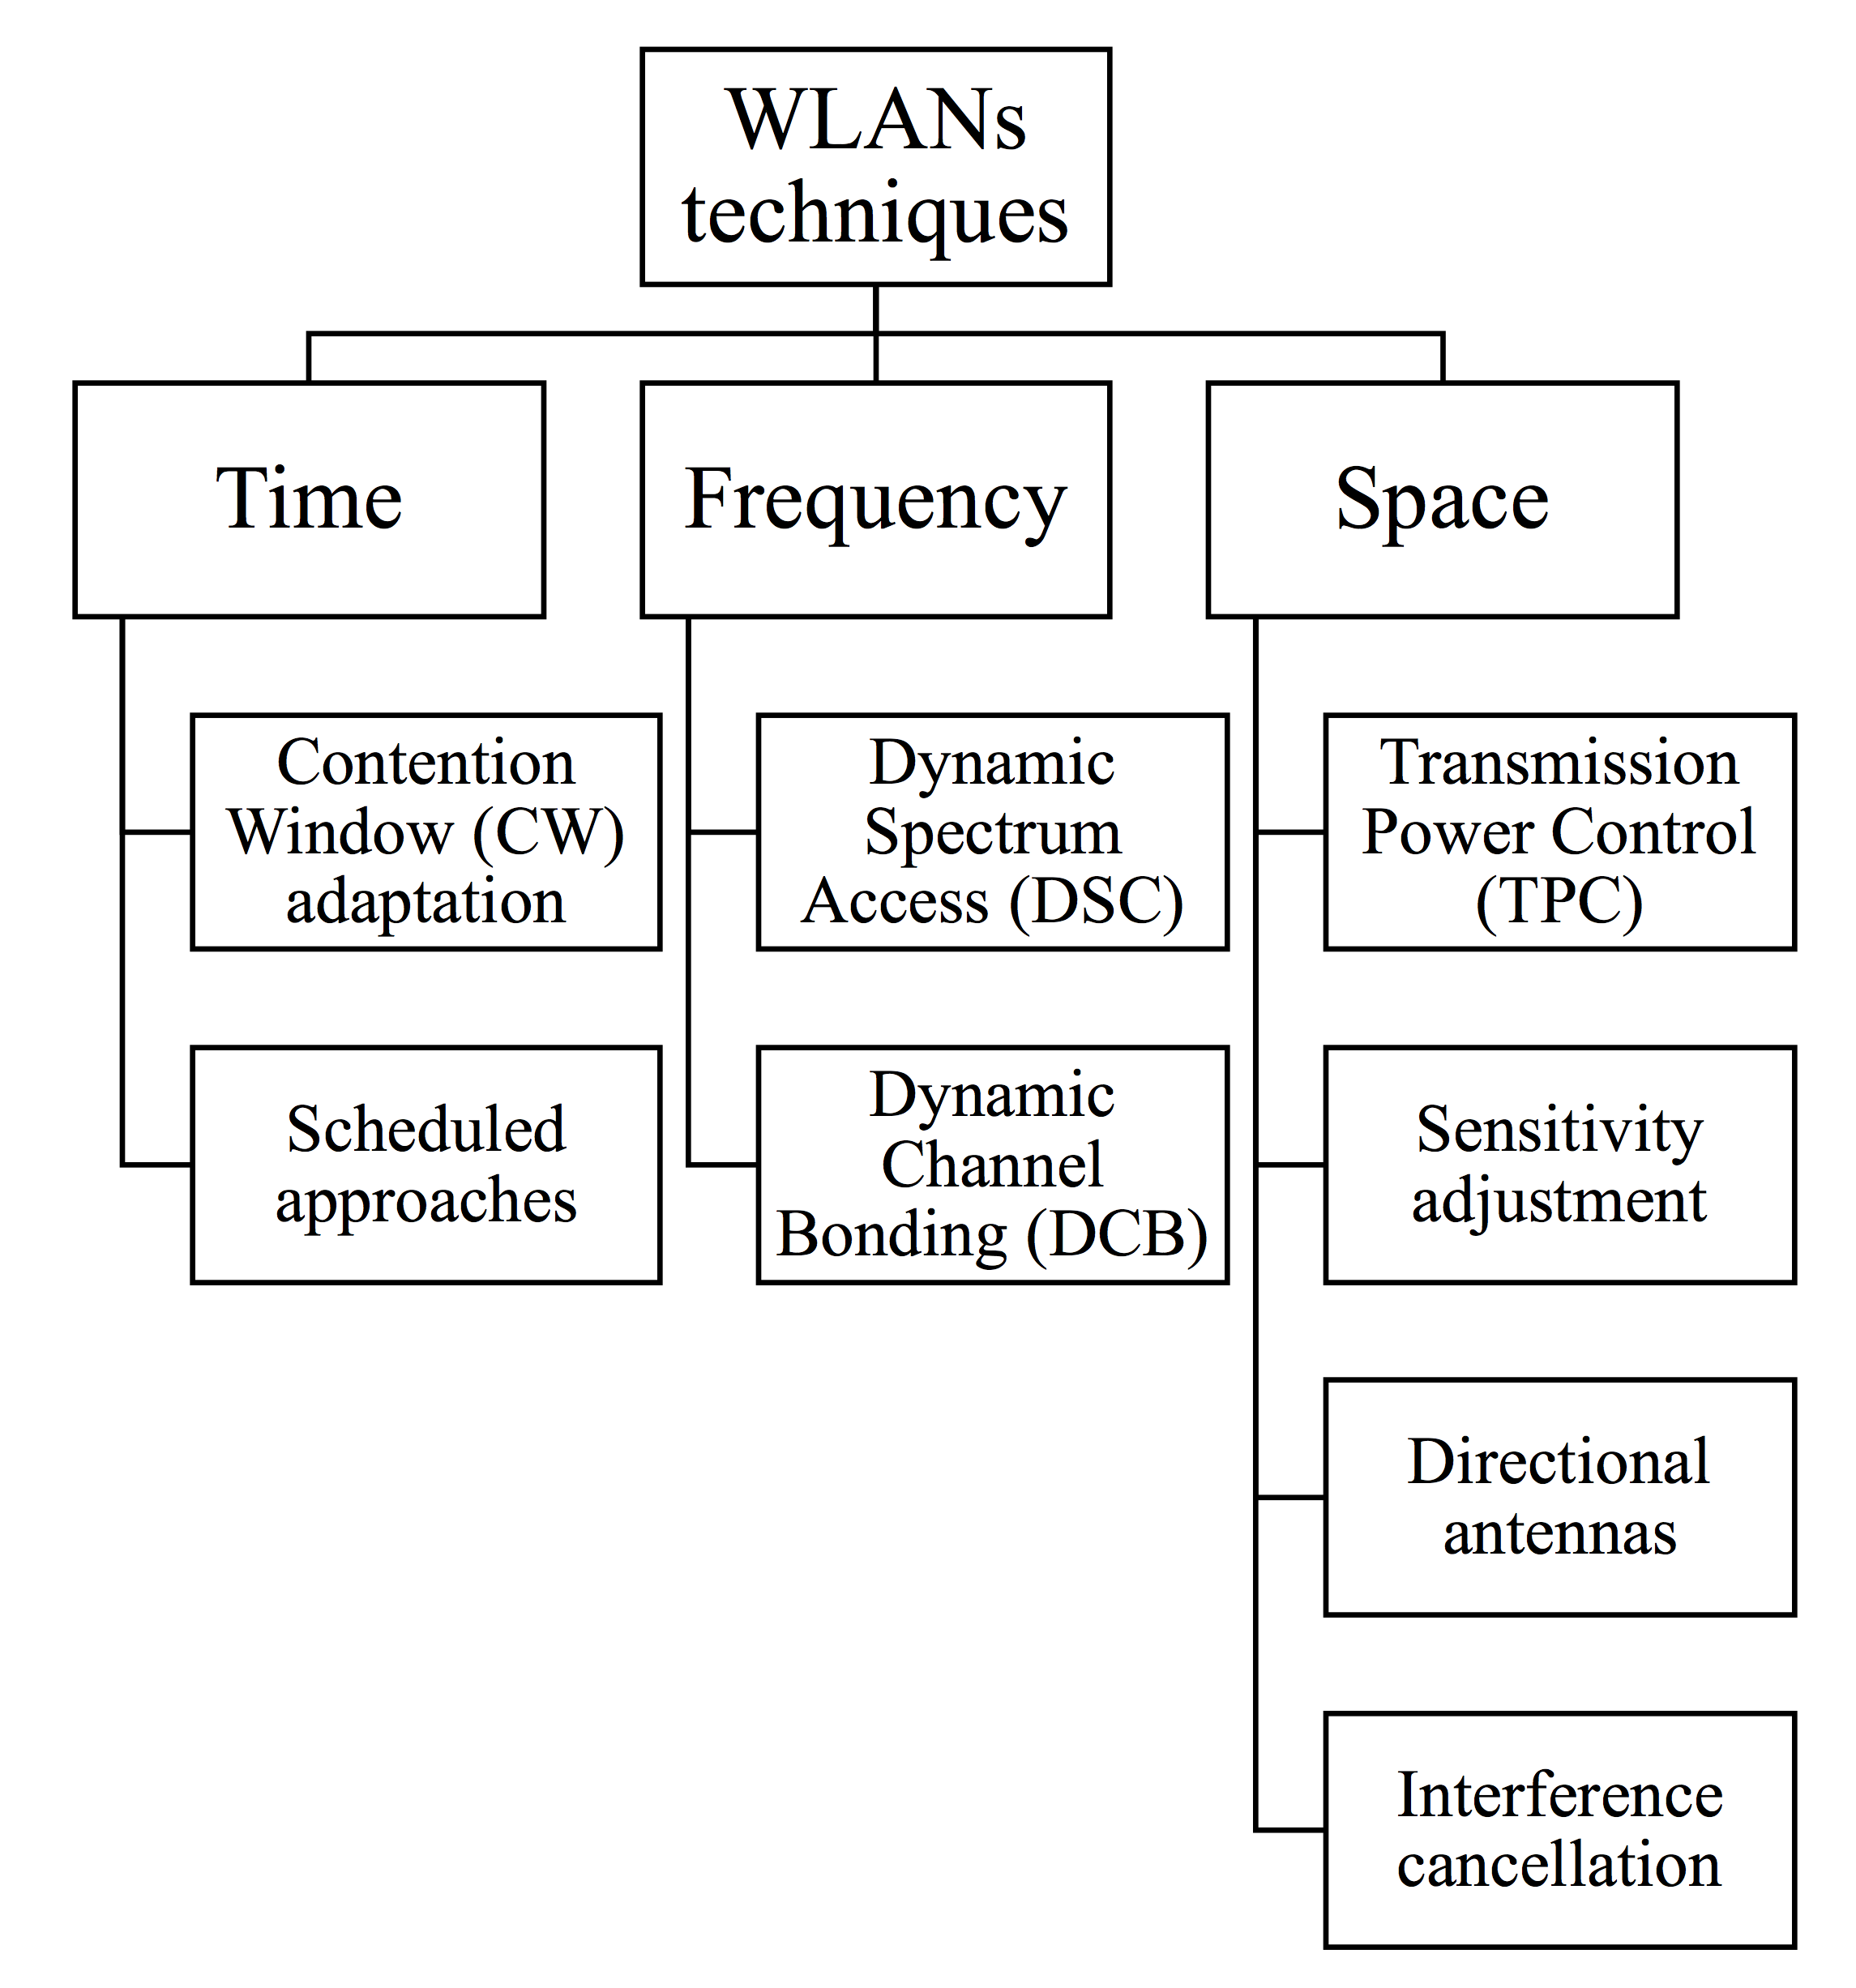
\epsfig{file=images/techniques_wns.png, width=10cm}
				\caption{Techniques to enhance WLANs performance}
				\label{fig:techniques_wns}
			\end{figure}	
			%The IEEE 802.11ax-2019 also includes many other novel mechanisms such as Orthogonal Frequency-Division Multiple Access (OFDMA), Dynamic Channel Bonding (DCB), and Multi-User Multiple Input Multiple Output (MU-MIMO). 
		
		\section{Contributions}
		\label{section:contributions}
			Given the problems regarding future WNs, the expected contributions of this thesis are:
			\begin{itemize}
				\item Understanding the challenges and limitations in future WLANs, thus allowing other researchers to deeply understand the subject and provide new solutions.
				\item Exploring the feasibility of applying Artificial Intelligence (AI) techniques into the spatial reuse problem in WNs.
				\item For the previous contribution, it is also expected to provide a simulation tool that allows the usage of intelligent agents.
				\item Providing solutions to the spatial reuse problem through learning approaches.
			\end{itemize}		
			
		The remainder of this document is structured as follows: Section \ref{section:research_problem} presents the Research Problem, as well as open challenges regarding the spatial reuse problem in WNs. The related work is shown in Section \ref{section:state_of_the_art}, which also includes the current literature in the application of Reinforcement Learning (RL) to Wireless Communications. Then, Section \ref{section:current_contributions} presents the ongoing work and the current contributions to the matter of this thesis. Finally, the working plan and the expected goals are provided in Section \ref{section:future_work}.

	%%%%%%%%%%%%%%%%%%%%%%%%%%%%%%%%%%%%%%%
	% RESEARCH PROBLEM							      %%%%%%%%%%%%%
	%%%%%%%%%%%%%%%%%%%%%%%%%%%%%%%%%%%%%%%
	\chapter{Research Problem}
	\label{section:research_problem}
		In this Section we describe the current issues and open challenges for the spatial reuse problem in overlapping WNs. To narrow the problem characterisation, IEEE 802.11 Wireless Local Area Networks (WLANs) are particularly focused.
		
		%%%%%%%%%%%%%%%%%%%%%%%%%%%%%%%%%%%%%%%
		% COEXISTENCE ISSUES						      %%%%%%%%%%%%%
		%%%%%%%%%%%%%%%%%%%%%%%%%%%%%%%%%%%%%%%
		\section{Coexistence Issues in IEEE 802.11 WLANs}
		\label{section:coexistence_issues}	
			Devices in IEEE 802.11 WLANs implement the Distributed Coordination Function (DCF) for accessing to the channel in presence of other nodes. DCF combines Carrier Sense Multiple Access with Collision Avoidance (CSMA/CA) with Binary Exponential Backoff (BEB). With that, before a packet transmission, a station listens to the channel for a period called Distributed Inter Frame Space (DIFS). Channel is sensed to be free according to the Clear Channel Assessment (CCA) mechanism, i.e., if the power sensed is lower than a given threshold. The power received at a given node is the sum of all the interference generated by the other devices under the environment-constrained propagation effects. Regarding BEB, it aims to reduce the number of potential collisions by randomizing the access to the channel, and by adapting the opportunities for accessing to it. In BEB, each station selects a random backoff value to start a countdown that prevents to transmit until it has been exhausted, thus minimizing collisions. In case channel is sensed as busy, the countdown is paused. It is resumed as soon as the ongoing transmission finishes and the channels is sensed as free again. Note that the backoff is a uniformly distributed random variable between 0 and the Contention Window (CW), which is doubled in case of noticing a packet failure until reaching a maximum value $\text{CW}_{max}$. The probability of noticing a collision decreases as CW increases, but this supposes that channel is free more time (also leading into throughput degradation).
					
			Despite the current mechanisms for allowing coexistence in WNs, and due to the nature of the CSMA/CA protocol, networks overlapping still drives into many problems and situations that result into poor throughput performance. In particular, there is a trade-off between the collisions occurring in an OBSS, the time channel remains idle, and the overhead generated to avoid harmful situations. In all the cases, both throughput and fairness in the WN are compromised. Two well-known problems often occur in IEEE 802.11 coexisting deployments, which are to a matter of interest for the research community. The first one, the Exposed-Terminal problem (or exposed node problem), occurs when a device is prevented to transmit due to the sensed interferences caused by other nodes, so that the CCA threshold is exceeded. Thus, throughput is reduced according to the number of exposed nodes that are sharing the same channel. On the other hand, the Hidden-Terminal node may generate collisions if two out-of-range nodes transmit at the same time to a node that senses both of them. In this case, the performance is affected by a higher collision probability, which may entail severe issues to several levels of the network architecture, such as routing or transport. Figure \ref{fig:hidden_exposed} shows both Hidden and Exposed Terminal Problems.					
			\begin{figure}[h!]
				\centering
				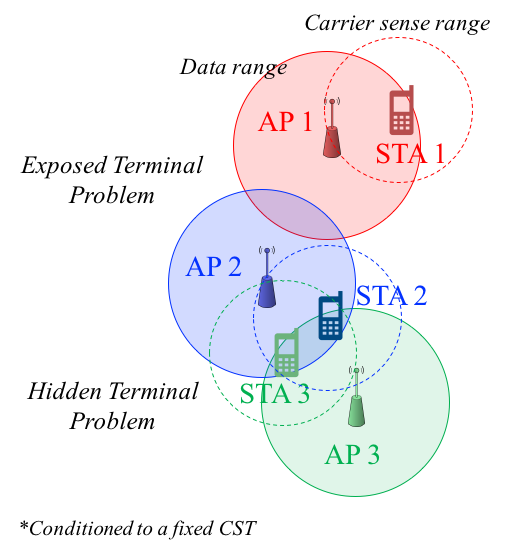
\epsfig{file=images/hidden_exposed.png, width=10cm}
				\caption{Exposed Terminal Problem: AP1 and AP2 could transmit simultaneously since STA1 and STA2 are enough away from the interference, but only a transmission at a time is allowed due to CSMA/CA. Hidden Terminal Problem: AP2 and AP3 may suffer collisions by hidden node because they are not in range each other, but STA2 and STA3 do.}
				\label{fig:hidden_exposed}
			\end{figure}		
			
			The hidden-terminal problem has been previously studied in \cite{ekici2008ieee, jang2012ieee}, which show performance loss in typical wireless deployments with moderate traffic. In order to minimise the hidden-terminal problem, the IEEE 802.11 amendment includes the optional Request-to-Send/ Clear-to-Send (RTS/CTS) mechanism. It basically consists in pre-allocating the channel before performing a data transmission. To do so, both source and destination interchange RTS and CTS frames in case the channel is sensed as free from both locations. Thus, potential hidden nodes go into a virtual carrier-sensing mode in case of listening any of the two frames. The Network Allocation Vector (NAV) is responsible to handle this virtual sensing. Figure \ref{fig:dcf_operation} shows the DCF operation with RTS/CTS.					
			\begin{figure}[h!]
				\centering
				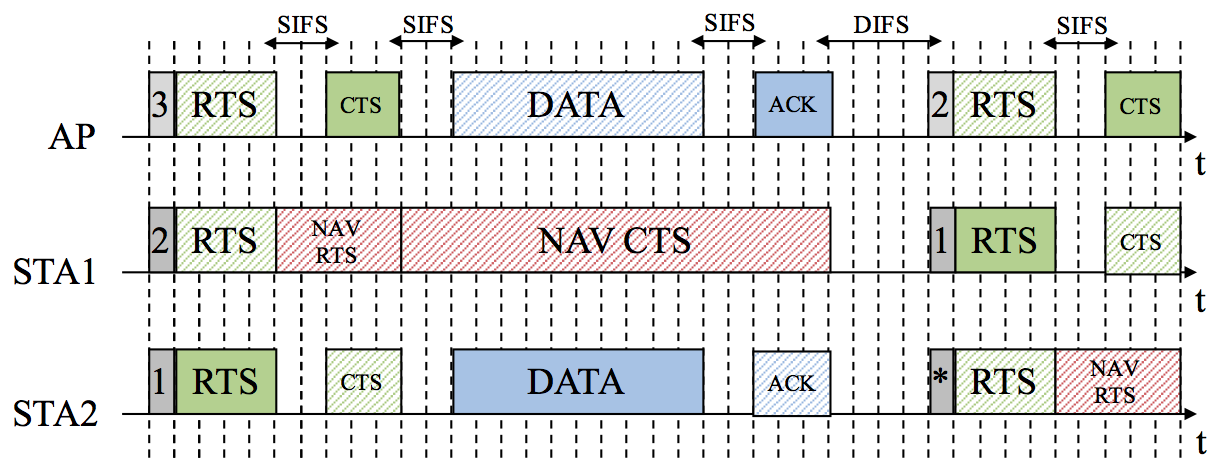
\epsfig{file=images/dcf_operation.png, width=14cm}
				\caption{DCF operation with RTS/CTS. After waiting 1 slot, STA2 sends an RTS frame to indicate that it wants to reserve the channel. A CTS frame is replied from the AP, so NAV is updated in STA1 to cover the entire transmission, as well as it operates at the same frequency channel.}
				\label{fig:dcf_operation}
			\end{figure}
			Despite the apparent enhancement provided by RTS/CTS, it may fail at solving the hidden-terminal problem. Firstly, either RTS and CTS frames may be not heard by interfering nodes. Furthermore, some counter productive effects are well-known to occur \cite{sobrinho2005rts}. In particular, performance anomalies are likely to occur in case of existing asymmetric links, which appear from the usage of different transmit powers and carrier sense thresholds.
					
		%%%%%%%%%%%%%%%%%%%%%%%%%%%%%%%%%%%%%%%
		% SCENARIOS												   %%%%%%%%%%%%%
		%%%%%%%%%%%%%%%%%%%%%%%%%%%%%%%%%%%%%%%						
		\section{Scenarios}
		\label{section:scenarios}	
		According to \cite{bellalta2016ieee}, next-generation WLANs will lead to dense scenarios, containing a high number of wireless devices (e.g. 1 user/m$^2$). Typical dense scenarios are provided by the IEEE 802.11ax amendment:
		\begin{itemize}			
			\item \textbf{Residential Scenario:} this scenario aims to characterise a typical uncoordinated deployment of WLANs, combining HEW and legacy devices. It consists in a 5-floors building of $3 m$ per floor (see Figure \ref{fig:building}), containing $2 \times 10$ apartments, which have size $10 m \times 10 m \times 3 m$ (see Figure \ref{fig:floor}). An indoor path-loss model is used to capture the effect of walls and other obstacles on the propagated signals. 
			\begin{figure}[h!]
				\centering
				\begin{subfigure}[b]{0.4\textwidth}
					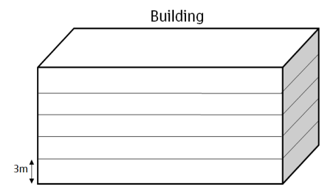
\includegraphics[width=\textwidth]{images/residential_ax_1}
					\caption{Building layout}
					\label{fig:building}
				\end{subfigure}
				\begin{subfigure}[b]{0.4\textwidth}
					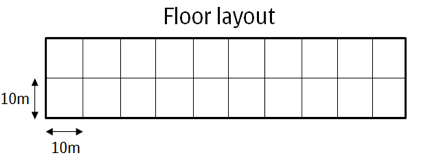
\includegraphics[width=\textwidth]{images/residential_ax_2}
					\caption{Floor layout}
					\label{fig:floor}
				\end{subfigure}		
				\caption{IEEE 802.11ax Residential scenario}
				\label{fig:ax_residential_scenario}
			\end{figure}			
			\item \textbf{Enterprise Scenario:} in this case, it is presented a coordinated scenario in which devices are mostly controlled. It is composed by 8 offices (see Figure \ref{fig:offices}), containing 64 cubicles (see Figure \ref{fig:cubicles}). In each office there are 4 APs installed in a mesh topology, and each cubicle contains 4 STAs (laptop, monitor, smartphone or tablet, and hard disk). The interference generated in such scenario is provided by the overlapping ESSs and unmanaged networks (P2P links). The path-loss considered takes into account the walls of the offices.
			\begin{figure}[t!]
				\centering
				\begin{subfigure}[b]{0.4\textwidth}
					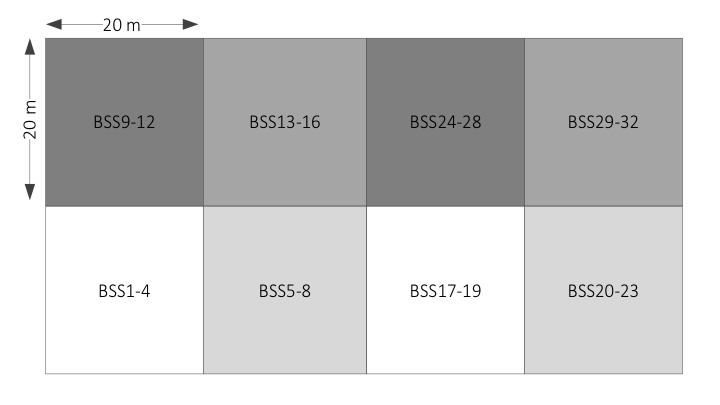
\includegraphics[width=\textwidth]{images/enterprise_ax_1}
					\caption{Offices layout}
					\label{fig:offices}
				\end{subfigure}
				\begin{subfigure}[b]{0.4\textwidth}
					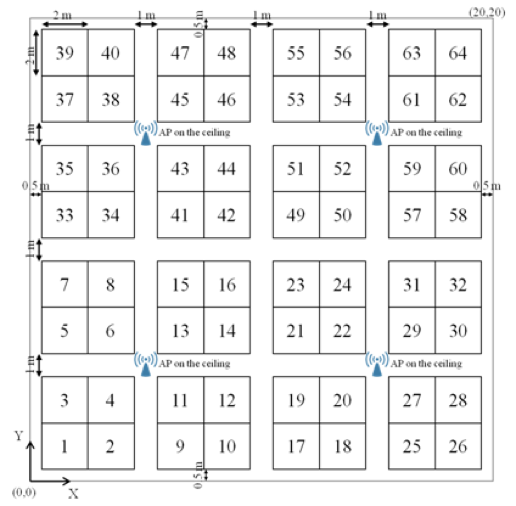
\includegraphics[width=\textwidth]{images/enterprise_ax_2}
					\caption{Cubicles layout}
					\label{fig:cubicles}
				\end{subfigure}		
				\caption{IEEE 802.11ax Enterprise scenario}
				\label{fig:ax_enterprise_scenario}
			\end{figure}
		
			\item \textbf{Indoor Small BSS  Scenario:} this scenario aims to represent coordinated real-world deployments that aim to extend mobile networks. To support a high number STAs, many long-range APs are placed. The ESS architecture is therefore planned through a given frequency reuse pattern (see Figure \ref{fig:large_ax}). The radius of each cell has size $10 m$, and there are $2 \cdot h$ meters between consecutive BSSs, where $h=sqrt(R2-R2/4)$. The AP is placed at the centre of the cell.			

			\item \textbf{Outdoor Large BSS Scenario:} similarly to the indoor BSS scenario, the objective for the outdoor large BSS scenario is to capture issues in real-world outdoor deployments with a high separation between BSSs. Again, the deployment is planned, so as the frequency reuse. The scenario is composed by 19 hexagonal grids, with an inter-AP separation of 130m. STAs are placed randomly through a uniform distribution, so that they associate to the nearest AP based on distance-based path loss and shadowing.  
			\begin{figure}[h!]
				\centering
				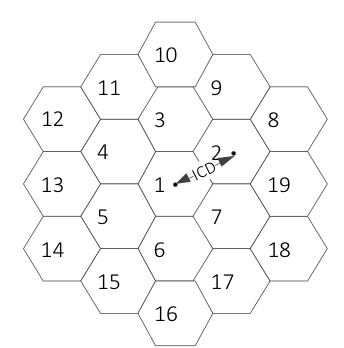
\epsfig{file=images/large_ax.png, width=5cm}
				\caption{IEEE 802.11ax Cell topologies}
				\label{fig:large_ax}
			\end{figure}	
		
			\item \textbf{Residential Scenario + Outdoor Large BSS Scenario:} it is a combination of the residential and the outdoor scenarios, so that different path-loss models are considered due to walls penetration in the building case.
			\begin{figure}[h!]
				\centering
				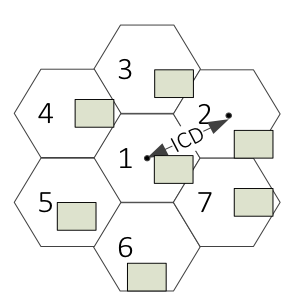
\epsfig{file=images/residential_large_ax.png, width=5cm}
				\caption{IEEE 802.11ax Residential + Large Outdoor BSS scenario}
				\label{fig:residential_large_ax}
			\end{figure}	
		\end{itemize}	
		In addition to the high density of nodes in the aforementioned scenarios, the variability in WNs in terms of user arrivals and departures entails an extra challenge to the resource allocation problem. Thus, adaptable and fast-convergence solutions must be provided, which even increases the problem complexity. Henceforth, the dynamic adjustment of parameters such as the frequency channel, the transmit power, or the sensitivity, appears to suit properly into the Reinforcement Learning (RL) paradigm (further described in Section \ref{section:rl}). In RL, input signals are used to determine the behaviour of a given system, so that historical events are considered for decision-making. To validate a real-time solution, it is very important to build an accurate model that takes into account the users behaviour. Thus, considering arrivals and departures is key for designing a solution, which must be provided before the environment changes. In both \cite{balachandran2002characterizing} and \cite{papadopouli2005modeling}, user arrivals are modelled as time-varying Poisson processes, such that the users arrival rate ($\lambda$) depends on the time. On these works, it is studied the users' behaviour in fully controlled environments such as a University Campus or a Conferences, but the mean time between user arrivals varies according to the scenario and many other factors. In particular, \cite{papadopouli2005modeling} considers a two-state Markov-Modulated Poisson Process (MMPP) with mean inter-arrival times of 38 seconds and 6 minutes for accessing and leaving the system, respectively. This gives us some notions about the requirements in terms of convergence time. In addition to scenarios diversification, it should be considered what will be the users behaviour in the future, as well as the algorithms to be designed must operate in the long term. 
			
		%%%%%%%%%%%%%%%%%%%%%%%%%%%%%%%%%%%%%%%
		% SPATIAL REUSE										     %%%%%%%%%%%%%
		%%%%%%%%%%%%%%%%%%%%%%%%%%%%%%%%%%%%%%%			
		\section{Spatial Reuse in Overlapping IEEE 802.11 WLANs}
		\label{section:spatial_reuse}	
			Spatial reuse aims to efficiently use the spectrum available regarding a limited area, specially in dense wireless deployments. To that purpose, we find Transmission Power Control (TPC), Carrier Sense Threshold (CST) adjustment, and beamforming. For the former, by adjusting the transmit power, the number of exposed nodes can be minimised, allowing a higher number of parallel transmissions within the same range. But there is an important consideration at tuning the power transmitted, which is that data rate directly depends on the SINR sensed at the receiver (the less power transmitted, the less experienced data rate received). Thus, adjusting TPC poses the trade-off between the number of parallel transmissions and the quality of them. Moreover, an insufficient transmit power may be unheard at the receiver, leading into packet losses. In addition, TPC can help at reducing energy consumption. Regarding CST adjustment, the number of parallel transmissions can be also be enhanced, in addition to a minimisation of the collisions probability by hidden-node. However, modifying the CST entails several consequences. For instance, decreasing the CST may rise probability of finding hidden nodes (the less is listened, the less is known). Table \ref{tbl:cca_tpc_effects} summarises the effects of TPC and CST adaptation.			
			\begin{table}[h!]
				\centering
				\begin{tabular}{|c|c|c|c|c|}
					\hline
					\multirow{2}{*}{\begin{tabular}[c]{@{}c@{}}\\ \textbf{Action}\end{tabular}} & \multicolumn{4}{|c|}{\textbf{Effect}} \\ \cline{2-5} 
					& \begin{tabular}[c]{@{}c@{}}Parallel\\ Transmissions\end{tabular}  & Data Rate & \begin{tabular}[c]{@{}c@{}}Collisions probability\\ (by hidden node)\end{tabular} & \begin{tabular}[c]{@{}c@{}}Energy\\ Consumption\end{tabular}\\ \hline
					$\uparrow$ Power & $\downarrow$ & $\uparrow$ & $\downarrow$ & $\uparrow$ \\ \hline
					$\downarrow$ Power & $\uparrow$ & $\downarrow$ & $\uparrow$ & $\downarrow$ \\ \hline
					$\uparrow$ CCA & $\downarrow$ & - & $\downarrow$ & $\downarrow$* \\ \hline
					$\downarrow$ CCA & $\uparrow$ & - & $\uparrow$ & $\uparrow$* \\ \hline
				\end{tabular}
				\caption{Effects of TPC and CST adjustment. \textit{*Adjusting CCA may indirectly affect to the energy consumption by requiring more/less power to be transmitted.}}
				\label{tbl:cca_tpc_effects}
			\end{table}
			Finally, to even improve spatial reuse we find adaptive beamforming, a technique that allows transmitting an energy beam into a specific direction. Thus, the usage of beamforming reduces the interference area for a given transmission. Figure \ref{fig:beamforming} shows how beamforming allows enhancing the spatial reuse through directional transmissions. In \ref{fig:beamforming1}, AP1 and AP2 cannot transmit simultaneously in case of using the same frequency channel, since they are using omnidirectional antennas. However, in case of using adaptive beamforming (\ref{fig:beamforming2}), the network throughput is doubled due to the parallel transmission from AP1 and AP2 to STA1 and STA2, respectively.
			\begin{figure}[t!]
				\centering
				\begin{subfigure}[b]{0.4\textwidth}
					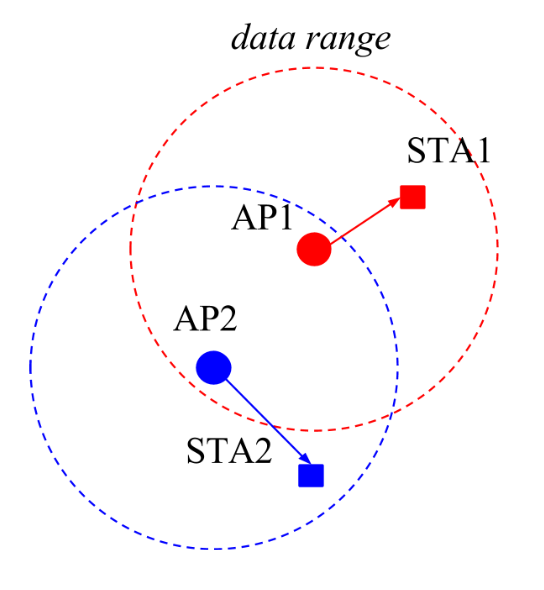
\includegraphics[width=\textwidth]{images/beamforming1}
					\caption{Omnidirectional transmission}
					\label{fig:beamforming1}
				\end{subfigure}
				\begin{subfigure}[b]{0.31\textwidth}
					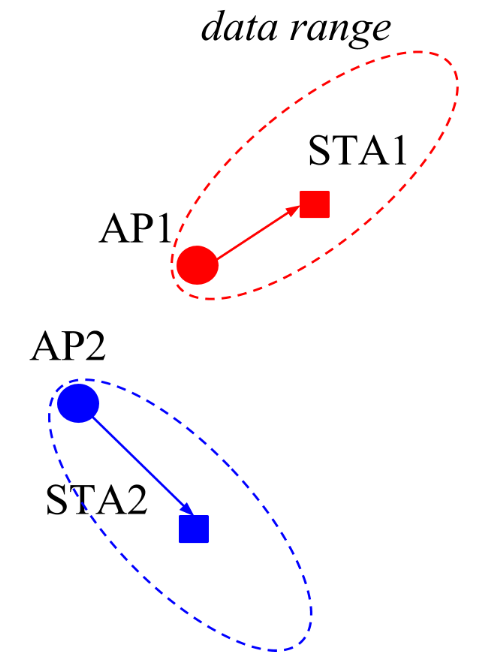
\includegraphics[width=\textwidth]{images/beamforming2}
					\caption{Directional transmission}
					\label{fig:beamforming2}
				\end{subfigure}		
				\caption{Enhancement of the spatial reuse through adaptive beamforming}
				\label{fig:beamforming}
			\end{figure}
						
		%%%%%%%%%%%%%%%%%%%%%%%%%%%%%%%%%%%%%%%
		% RL VISION									     		%%%%%%%%%%%%%
		%%%%%%%%%%%%%%%%%%%%%%%%%%%%%%%%%%%%%%%			
		\section{Autonomous Management in Wireless Networks}
		\label{section:rl_vision}
			For a proper operation in future WNs, we envision the usage of AI techniques to satisfy the high-demanding requirements in the complex scenarios abovementioned in Section \ref{section:scenarios}. The recent literature shows an upward trend in combining AI with Wireless Communications to solve many well-known problems such as packet routing \cite{littman1993distributed}, IEEE 802.11 WLAN Access Point Selection \cite{bojovic2011supervised, bojovic2012neural}, optimal rate sampling \cite{combes2014optimal}, or energy harvesting in heterogeneous networks \cite{miozzo2015distributed}. For the particular case of modifying the transmit power and the CST, finding the optimal solution in real time is NP-hard. For that, we put special emphasis on RL for improving the spatial reuse in high-density WNs. RL turns out to be a convenient paradigm for allowing independent devices to improve their own performance through an observations-based learning process.
			
	%%%%%%%%%%%%%%%%%%%%%%%%%%%%%%%%%%%%%%%
	% STATE OF THE ART				                 %%%%%%%%%%%%%
	%%%%%%%%%%%%%%%%%%%%%%%%%%%%%%%%%%%%%%%	
	\chapter{State of the Art}
	\label{section:state_of_the_art}
		This Section describes the current literature on spatial reuse enhancement in Wireless Networks, which embraces channel allocation, TPC, CST adjustment and beamforming. Since one of the main purposes of this thesis is to study the feasibility of RL application into spatial reuse in wireless networks, we also provide some notions on what RL is, and which kind of problems it can solve. Furthermore, in this Section we also introduce previous research in dynamic resource allocation in WNs through RL. 
			
		%%%%%%%%%%%%%%%%%%%%%%%%%%%%%%%%%%%%%%%
		% SoA DCA										          %%%%%%%%%%%%%
		%%%%%%%%%%%%%%%%%%%%%%%%%%%%%%%%%%%%%%%				
		\section{Dynamic Channel Allocation}		
		\label{section:dca}					
			Despite Dynamic Channel Allocation (DCA) is contained in the frequency domain, it is worth to study it in order to relax the spatial reuse problem. DCA aims to properly allocate the available frequency range among the overlapping devices, so that the interference can be notably reduced, and thus the aggregate throughput can be maximised. Because of the high traffic and users fluctuation experienced in wireless networks, DCA turns out to be necessary for improving the performance in a WN. Several DCA approaches can be found according to the needs, and there is a strong discussion about the requirements that must be accomplished. While some approaches aim to provide fairness (\cite{ling2006joint}), some others try to grant more resources to nodes with higher traffic demands (\cite{wertz2004automatic}). 	
		
			The Industrial, Scientific and Medical (ISM) band is shared by multiple technologies such as IEEE 802.11, IEEE 802.15 and Unlicensed Long Term Evolution (U-LTE). In particular, most of the Wi-Fi standards use the 2.4 GHz	and 5 GHz bands, which have different number of channels. For the 2.4 GHz case, there are 14 overlapping channels of 22 MHz (refer to Figure \ref{fig:channelisation_wifi}), so that adjacent channel utilisation ($\pm$ 11 MHz) is affected by a 30 dB signal drop (shown in Figure \ref{fig:80211ad_mask}). Similarly, the 5 GHz band is composed by three sub-bands, each one containing four non-overlapping channels. For using this band it is required to implement some mechanisms such as Dynamic Frequency Selection (DFS) or TPC.
			\begin{figure}[h!]
				\centering
				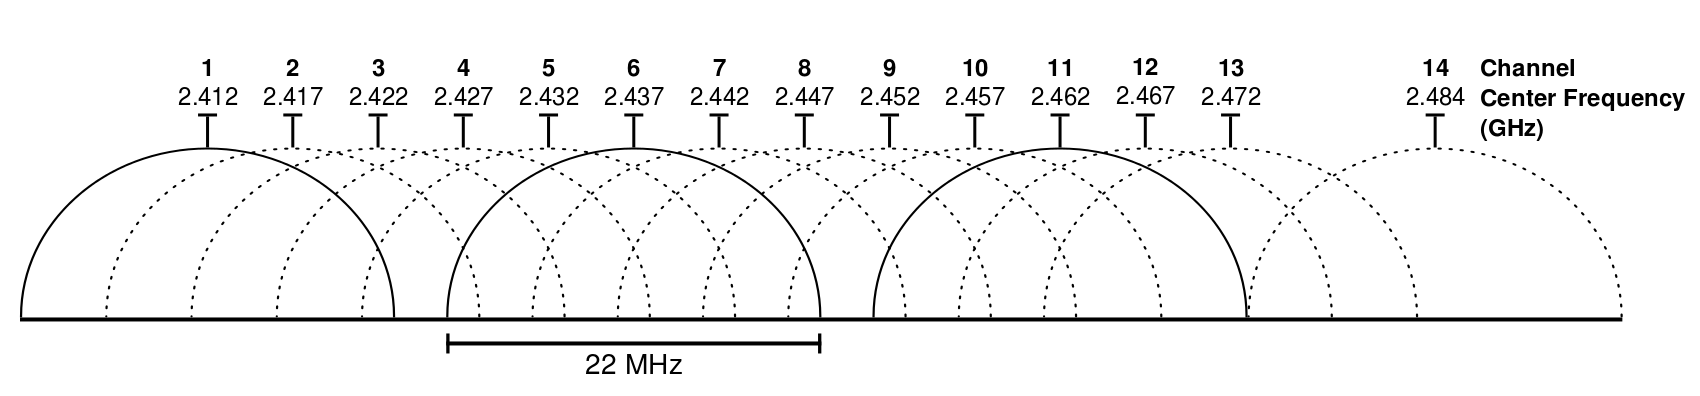
\epsfig{file=images/channelisation_wifi.png, width=15cm}
				\caption{Channelisation of the 2.4 GHz band}
				\label{fig:channelisation_wifi}
			\end{figure}
			\begin{figure}[h!]
				\centering
				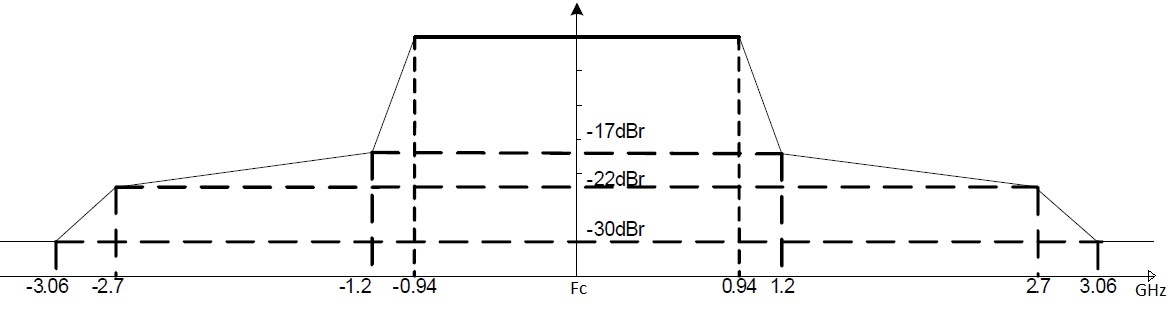
\epsfig{file=images/WLAN-802-11-spectrum-mask.jpg, width=11cm}
				\caption{IEEE 802.11 mask}
				\label{fig:80211ad_mask}
			\end{figure}			
			The saturation of the unlicensed band demands a proper channel allocation, which for dense deployments becomes a challenging task due to the scarce number of available non-overlapping channels. Thus, both frequency planning and dynamic channel selection have been of remarkable interest to the wireless communications community for enhancing the throughput area in overlapping WNs. A proper frequency planning allows reducing the interference between wireless devices, thus enhancing the overlapping networks capacity by avoiding collisions and delayed medium accesses. Dynamic channel selection allows wireless devices to change their centre frequency according to channel utilisation, which depends on the surrounding environment. A survey of channel assignment is provided in \cite{chieochan2010channel}, which introduced techniques are summarised in Tables \ref{tbl:channel_assignment_coordinated} and \ref{tbl:channel_assignment_uncoordinated}. Many of the reviewed techniques imply the existence of a central node that makes the channel assignment, which is infeasible for uncoordinated deployments like in the residential scenario. In contrast, decentralised mechanisms allow dynamic channel allocation based only on local information. However, many of them require from inter-AP communication and may lead to non-optimal solutions.
			\begin{table}[h!]
				\centering
				\begin{tabular}{llcc}
					\hline
					\multicolumn{1}{c}{\textbf{Technique}} & \multicolumn{1}{c}{\textbf{Description}} & \textbf{References} & \textbf{\begin{tabular}[c]{@{}c@{}}With AP \\ Placement\end{tabular}} \\ 
					\hline
					\begin{tabular}[c]{@{}l@{}}Graph \\ Colouring\end{tabular} & \begin{tabular}[c]{@{}l@{}}By assuming that APs are vertexes \\ and non-overlapping channels are\\ colours, graph colouring is applied to\\ minimise the interference between\\ adjacent cells. Graph colouring can be\\ also used for AP placement.\end{tabular} & \cite{hills2001large,mahonen2004automatic, riihijarvi2005frequency,riihijarvi2006performance} & Yes / No \\ \hline
					\begin{tabular}[c]{@{}l@{}}Integer Linear \\ Programming \\ (ILP)\end{tabular} & \begin{tabular}[c]{@{}l@{}}ILP is used to place APs and assign \\ channels by considering load balancing.\end{tabular} & \cite{lee2002optimization} & Yes \\ \hline
					\begin{tabular}[c]{@{}l@{}}Priority-Map \\ Approach\end{tabular} & \begin{tabular}[c]{@{}l@{}}A floor plan is divided into pixels, \\ which are assigned different priorities.\\ Then, both channel assignment and\\ AP placement is solved according to\\ built priorities.\end{tabular} & \cite{wertz2004automatic} & Yes \\ \hline
					\begin{tabular}[c]{@{}l@{}}Patching \\ Algorithm\end{tabular} & \begin{tabular}[c]{@{}l@{}}An heuristic algorithm is proposed\\ for maximising the throughput\\ and the fairness among wireless \\ clients, so that APs are being \\ sequentially placed according to \\ an objective function.\end{tabular} & \cite{ling2006joint} & Yes \\ \hline
					\begin{tabular}[c]{@{}l@{}}Coverage-\\ Oriented \\ Approach\end{tabular} & \begin{tabular}[c]{@{}l@{}}Linear programming is used to \\ optimise channel assignment and\\ AP placement, so that two objective\\ functions are used to that purposes.\end{tabular} & \cite{eisenblatter2007integrated} & Yes \\ \hline
					\begin{tabular}[c]{@{}l@{}}Conflict-free\\ Set Colouring\end{tabular} & \begin{tabular}[c]{@{}l@{}}Optimal AP association is provided \\ to minimise the interference\end{tabular} & \cite{mishra2006client} & No \\ \hline
					\begin{tabular}[c]{@{}l@{}}Measurement-\\ based local \\ coordination\end{tabular} & \begin{tabular}[c]{@{}l@{}}Both APs and clients need to measure\\ the interference sensed in all the \\ frequency channels in order to derive\\ an optimal solution for channel\\ assignment.\end{tabular} & \cite{chen2007improved} & No\\ \hline
				\end{tabular}
				\caption{Coordinated approaches for channel assignment}
				\label{tbl:channel_assignment_coordinated}
			\end{table}
			
			Centralised (or coordinated) approaches allow to effectively provide optimal (or close-to-optimal) solutions to the channel assignment problem, since complete knowledge and control on the network is granted. Moreover, in \cite{baid2015understanding} it is shown that centralised approaches allow to significantly improve the performance of a network, even with the existence of independent devices. To make centralised channel allocation, the first related literature that we find is based in graph colouring techniques. In contrast, even if centralised approaches are used, graph colouring is an NP-hard problem, which makes from it an infeasible solution for large scale scenarios. To solve that, we find several works that use heuristics in practical applications. The authors in \cite{brelaz1979new} firstly introduced the DSATUR algorithm for that purpose, which models the frequency allocation problem using interference graphs, so that higher-degree nodes have preference at choosing their centre frequency. An extension of DSATUR is found in \cite{villegas2009frequency}, which includes packet losses and co-channel interference in the decision-making process. In this case, the degree of a node is not given by its connections, but also by the interference and the utilisation. Several architectures are provided for running the algorithm, but all of them entail a full communication between nodes, so centralisation is required. Another fully centralised approach is introduced by \cite{raniwala2004centralized} in the context of wireless mesh networks, showing improvements of factor 2.63 in real scenarios (wireless cards are used to run the channel assignment algorithm based on the load). To do so, the authors propose a load-aware algorithm for dynamic channel selection, so traffic information is required in before-hand to provide a new channels configuration. 
			
			\begin{table}[h!]
				\centering
				\begin{tabular}{llc}
					\hline
					\multicolumn{1}{c}{\textbf{Technique}} & \multicolumn{1}{c}{\textbf{Description}} & \textbf{References} \\ \hline
					\begin{tabular}[c]{@{}l@{}}Least Congested\\ Channel Search\\ (LCCS)\end{tabular} & \begin{tabular}[c]{@{}l@{}}APs listen to all the channels and select\\ the one with lowest sensed interference.\\ Other parameters such as traffic \\ information is also used to make a \\ decision.\end{tabular} & \cite{achanta2004method} \\ \hline
					\begin{tabular}[c]{@{}l@{}}MinMax\\ Approaches\end{tabular} & \begin{tabular}[c]{@{}l@{}}Based on the assumption that heavily\\ loaded APs degradate the network\\ performance, MinMax aims to minimise\\ the maximum effective channel \\ utilisation of those devices.\end{tabular} & \cite{leung2003frequency,yu2006dynamic,yu2004adaptive} \\ \hline
					\begin{tabular}[c]{@{}l@{}}Weighted\\ Colouring\end{tabular} & \begin{tabular}[c]{@{}l@{}}From the devices' perspective, it is \\ used the sensed interference and the \\ number of overlapping devices to \\ minimise an objective function that leads\\ to channel assignment.\end{tabular} & \cite{mishra2005weighted} \\ \hline
					\begin{tabular}[c]{@{}l@{}}Pick-rand and\\ Pick-first\end{tabular} & \begin{tabular}[c]{@{}l@{}}Based on the sensed interference, a new\\ channel is chosen randomly or according\\ to a ranking list (based also on the power\\ sensed).\end{tabular} & \cite{akl2007dynamic,haidar2007channel, al2007enhanced}\\ \hline
					\begin{tabular}[c]{@{}l@{}}Channel\\ Hopping\end{tabular} & \begin{tabular}[c]{@{}l@{}}APs change their channel periodically in\\ order to maximise the throughput in a\\ long run.\end{tabular} & \cite{mishra2006distributed} \\ \hline
				\end{tabular}
				\caption{Uncoordinated approaches for channel assignment}
				\label{tbl:channel_assignment_uncoordinated}
			\end{table}
			
			Centralised approaches have been shown to be very effective at maximising network performance in overlapping environments by providing a proper channel allocation. However, several limitations are found in real world. Firstly, many overlapping wireless deployments are independent, so they cannot be managed by a central entity. In addition, the required underlying communication adds a higher degree of complexity, which solution may lead to counter productive overhead. For that, we aim to focus on decentralised approaches (with and without communication), which allow facing the channel allocation problem in a simpler way in terms of synchronisation. Furthermore, for the cases in which communication is required, we are interested in quantifying the generated overhead in order to notice the actual improvements achieved. Regarding decentralised mechanisms for channel assignment, we first focus on \cite{mishra2005weighted}, which presents a weighted colouring approach to improve the resources sharing problem in overlapping WNs. In particular, two techniques are provided, which are $i)$ fully decentralised and $ii)$ based on messaging passing. Again, the channel assignment problem in WLANs is approached through graph colouring, providing edges to nodes that suffer from neighbouring interference. The goal is to assign colours (i.e., channels) to nodes, so that adjacent nodes use different channels, and at the same time their usage is minimised. The fact of experiencing co-channel interference makes from this a weighted colouring problem, so an objective function is provided. This function aims to minimise the interference suffered by devices in an overlapping network. To allow decentralisation, the algorithm can only attempt to minimise the interference of a given AP, which ends up to reducing the total interference if the network progressively adjusts itself as a whole. A step further to provide fast-convergence and better results in terms of interference, is to centralise the algorithm by considering the aggregate interference. For that, a reliable communication between APs must be carried out. Notwithstanding, the implication of this communication is not even mentioned in this work, so it is not possible to determine if the presented method is practical due to the overhead or even feasible. Furthermore, \cite{herzen2013distributed} shows that minimising the interference through an objective function is only worth for very dense scenarios, which lacks of flexibility for maximising the throughput area. To improve that, the authors present a fully decentralized approach through a minimisation function that takes into account the total sensed interference and a cost associated to the bandwidth utilisation. The sum of both measurements is referred as the \textit{energy}:
			\begin{equation}
			\mathcal{E} (\textbf{F},\textbf{B}) = \sum_{A \in \mathcal{A}} \sum_{B \in \mathcal{N}_A} I_A (B) + \sum_{A \in \mathcal{A}} cost_A (b_A)
			\end{equation}
			Where $I_A (B)$ is the interference sensed at BSS $A$, originated by the other WLANs $B \in \mathcal{N}_A$, and $cost_A (b_A)$ is the cost that BSS $A$ obtains from using bandwidth $b_A$. The algorithm works in the APs as follows:
			\begin{figure}[h!]
				\centering
				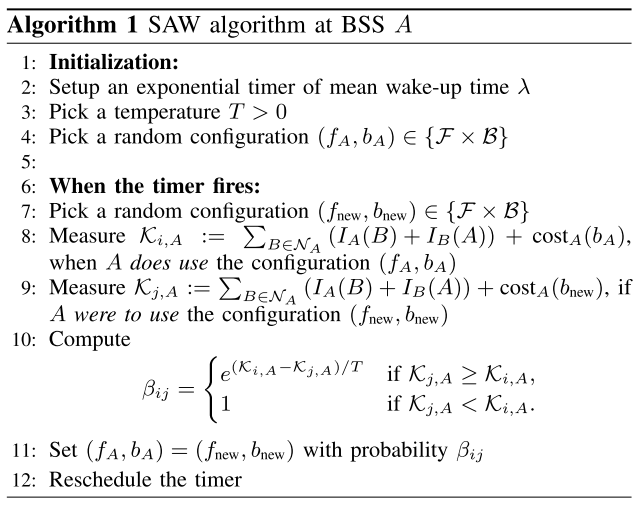
\epsfig{file=images/saw_alg.png, width=8cm}
				%\caption{}
				\label{fig:saw_alg}
			\end{figure}	
			The first experimental part (simulations carried out through Python) considers studying the modification of the cost function $c/b_A$ (where $c$ is a constant and $b_A$ is the bandwidth used by BSS $A$), so that different dynamics of the joint performance in the overlapping networks can be captured. For a null cost, the interference is attempted to be mitigated, which is shown to be effective for high densities. The opposite occurs for a larger value of $c$ (in this case, $c=100$), which is only useful to improve the capacity when few overlapping networks exist, but harms the overall performance in case density increases. In addition, fairness is shown to linearly decrease as $c$ increases. Then, a testbed implementation is provided by using 21 wireless nodes applying the channel allocation algorithm. It is shown a significant improvement for UDP and TCP traffic cases that overtakes the optimal performance achieved by applying frequency allocation through graph colouring.
								
			Other mechanisms for decentralised channel assignment that also rely in making measurements to enhance the network conditions, can be found in \cite{akl2007dynamic, chen2007improved}. \cite{akl2007dynamic} proposes a very simple approach in which the APs maintain an interference map of their neighbours, such that channel assignment can be done through interference minimisation. Unfortunately, neither interactions between APs due to decentralisation are studied, nor strong evidences for improvements are provided. Separately, \cite{chen2007improved} proposes two decentralised approaches (in addition to a centralised one) that rely in the interference measured at both APs and STAs to calculate the best frequency channels for dynamic channel allocation. The shown uncoordinated approach presents acceptable results at minimising the interference in an overlapping network. In addition, a coordinated approach with messaging passing is presented, enhancing previous results. The main drawback of the latter is the requirement of a wired infrastructure for the management communication, which is often infeasible, specially in typical residential scenarios. 				
			
			%%%%%%%%%%%%%%%%%%%%%%%%%%%%%%%%%%%%%%%
			% SoA TPC											      %%%%%%%%%%%%%
			%%%%%%%%%%%%%%%%%%%%%%%%%%%%%%%%%%%%%%%			
			\section{Transmit Power Control}
			\label{section:tpc}
				Adjusting the transmit power is another technique considered in the IEEE 802.11ax standard for spatial reuse enhancement. In the first version of the draft \cite{tgax2016draft}, a set of regulations are provided for TPC usage. In particular, when a STA chooses a specific power detection level ($\text{OBSS\_PD}_{level}$), the maximum transmit power is given by:						
				\begin{scriptsize}
					\begin{equation}
					\text{TX\_PWR}_{max}=
					\begin{cases}
					\text{Unconstrained}, & \text{if}\ \text{OBSS\_PD}_{level} = \text{OBSS\_PD}_{min} \\
					\text{TX\_PWR}_{ref}-(\text{OBSS\_PD}_{level}-\text{OBSS\_PD}_{min}), & \text{OBSS\_PD}_{max} \geq \text{OBSS\_PD}_{level} \geq \text{OBSS\_PD}_{min}
					\end{cases}
					\nonumber
					\end{equation}				
				\end{scriptsize}				
				Despite the context provided by the TGax, modifying the transmit power is a complex task that must be carefully done, since may affect to the higher communication layers such as network (routing) and transport (congestion). Due to the fact that transmission range and the data rate are conditioned by power control at the physical layer, the main effects of increasing the transmission power in a wireless network are:
				\begin{itemize}
					\item Generates more interference, which may cause a higher contention time for the overlapping nodes.
					\item Increases the data rate.
					\item Increases the transmission range, which is helpful for connectivity with the receiver but harmful for the overlapping nodes due to the generated interference.
					\item Increases the energy consumption.\footnote{Energy consumption is affected by the type of power consumption (power transmission, power idle, power sleep, power amplifier and power reception) and the devices involved in the communication. To apply a policy for saving power is strictly related to them, which is out of the scope of this Thesis.}
				\end{itemize}				
				Furthermore, TPC may create unidirectional links, which unleashes fairness issues within overlapping nodes. In fact, acknowledgements (ACKs) and RTS/CTS frames assume bidirectional links. To properly implement TPC, the first question to be asked is where should power control be done in the network architecture. This question is presented in \cite{kawadia2005principles}, which, in addition to devising that the network level should be in charge of power control, presents a guideline of its impact on several performance measures (end to end delay, packet losses, routing overhead, etc.). The authors claim that global optimization is carried out by TPC approaches acting in the network layer, rather than in the MAC layer. The latter only solves the transmit power control problem locally (usually, SINR is used to adjust power). Furthermore, TPC approaches acting in the MAC layer only aim to adjust power at the immediate hop, so that the next optimal hop problem is not considered (this is a very common issue in ad-hoc WNs).
				
				The first literature that proposes TPC is mainly focused on energy saving. Despite this topic is out of the scope of this work, it is interesting to study the kind of mechanisms used and the implementations done for that purpose. In \cite{agarwal2001distributed, karn1990maca} there are presented several power control schemes relying on the RTS/CTS mechanism. In them, these management packets are used to measure the power transmitted by the overlapping wireless devices. Thus, TPC can be done in such way that the number of parallel transmissions increases whilst collisions are minimised. However, it is known that these kind of schemes can degrade the network throughput and may even incur into a higher energy consumption \cite{ebert1999combined}. To solve that, \cite{pursley2000energy} proposes to adjust the transmit power only during data transmissions. It is used the minimum necessary to successfully carry out the transmission, which is also computed through the RTS/CTS frames. Furthermore, to avoid collisions, the devices in a wireless network have to use the maximum power ($p_{max}$) when transmitting either an RTS or a CTS frame. In particular, RTS/CTS frames are modified to include the current and the desired power transmitted at the transmitter and at the receiver, respectively. The desired power ($p_{desired}$) is adjusted as $p_{desired} = p_{max} \times Rx_{Thresh} \times c$, where $Rx_{Thresh}$ is the minimum necessary received signal strength and $c$ is a constant (which in this case is set to 1). Figure \ref{fig:basic_tpc} shows the behaviour of the power control scheme introduced in \cite{pursley2000energy}.	
				\begin{figure}[h!]
					\centering
					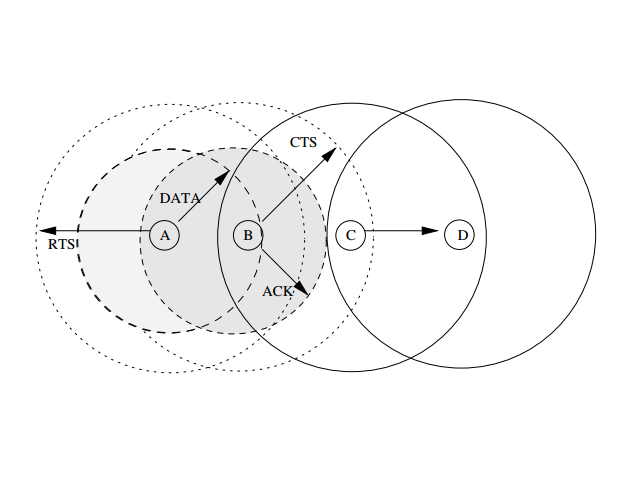
\epsfig{file=images/basic.png, width=8cm}
					\caption{Pursley et al. Power Control Scheme}
					\label{fig:basic_tpc}
				\end{figure}				
				A further extension of this work is presented in \cite{jung2002power}, as well as the power control scheme shown in \cite{pursley2000energy} may potentially decrease the throughput and increase energy consumption in some scenarios. The main root cause points out the collisions that may occur due to the Hidden-Node problem, since neither CTS nor RTS frames may not be listened by some interfering nodes. Therefore, the new proposed scheme, which is named Power Control MAC (PCM), deals with the aforementioned kind of asynchronies by forcing nodes to transmit periodically DATA at the maximum power. Figure \ref{fig:pcm} shows the power used during a DATA/ACK transmission if using PCM, which is set to $p_{max}$ during $20 \mu s$ every $190 \mu s$. These values are predefined because the EIFS value specified by the DCF is equal to $212 \mu s$ when the data rate is 2 Mbps. Thus, power level during DATA transmission is increased once in each EIFS interval.
				\begin{figure}[h!]
					\centering
					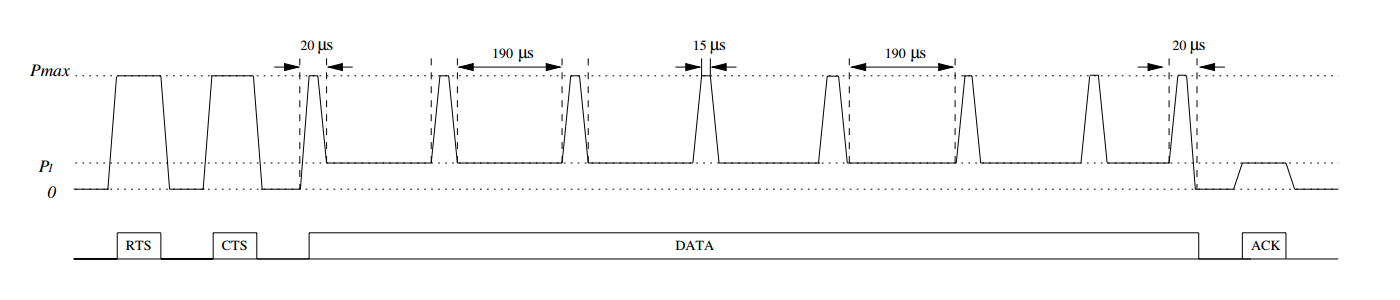
\epsfig{file=images/pcm.png, width=16cm}
					\caption{PCM Scheme}
					\label{fig:pcm}
				\end{figure}
				This power control scheme has been validated for several network topologies, so that remarkable improvements are shown at saving energy. In particular, savings of about 10\% are achieved whilst obtaining very similar throughput values with respect to current IEEE 802.11 operation. Despite the main goal of the PCM scheme used is to reduce energy consumption, it implicitly allows improving the spatial reuse, which shows that using the necessary power during a wireless transmission can be beneficial for the network capacity. Similarly to previous reviewed approaches that make use of RTS/CTS frames, the authors in \cite{lei2015performance} attempt to improve the throughput of OBSSs by using an RTS/CTS modification that incorporates different Network Allocation Vector (NAV) timers. Thus, despite RTS and CTS packets are transmitted at the maximum power, a higher number of parallel transmissions can be carried out, since the new NAV timers only captures the RTS/CTS operation. However, this solutions appears to be quite rigid and to behave properly only in few situations.
				
				Another important research line for TPC is based on measuring and/or inferring the channel characteristics. The authors in \cite{chaves2014adaptive} show the benefits of tuning the transmit power in terms of interference, and without affecting to the MCS granted by the Channel State Information (CSI) from previous transmissions. In \cite{oteri2013advanced}, the authors also study the potential of TPC. In particular, four TPC schemes are provided for theoretical comparison:
				\begin{itemize}
					\item No TPC: devices transmit at the maximum transmit power.
					\item Basic TPC: devices transmit at the minimum necessary power to reach the farthest device in their network.
					\item Unfiltered TPC: the power is adjusted to the minimum necessary per link communication, but beacons to the minimum required power for reaching the farthest device.
					\item Filtered TPC: an IIR filter is used to adjust the transmit power $y(n)$, which is computed as $y(n) = a \cdot y(n-1) + (1-a) \cdot x(n)$, where  $y(n-1)$ is the previous estimated transmit power, and $x(n)$ is the instantaneous power needed.
				\end{itemize}  
				Several experiments are done regarding the uplink and the downlink performance for several combinations of the introduced approaches, showing the potential of providing such kind of power control mechanism. In addition, it also introduces the concept of Fractional-CSMA/CA, which aims to coordinate the transmissions within different BSSs in order to make the most of TPC. Thus, the number of parallel transmissions can be increased without suffering collisions by hidden node (refer to Figure \ref{fig:fcsma}). The concept of F-CSMA/CA is also interesting to even improve the TPC operation, since it would allow to make a step further for enhancing spatial reuse. However, it requires a strong coordination that appears to be infeasible in the uncoordinated scenarios of interest for this work.
				\begin{figure}[t!]
					\centering
					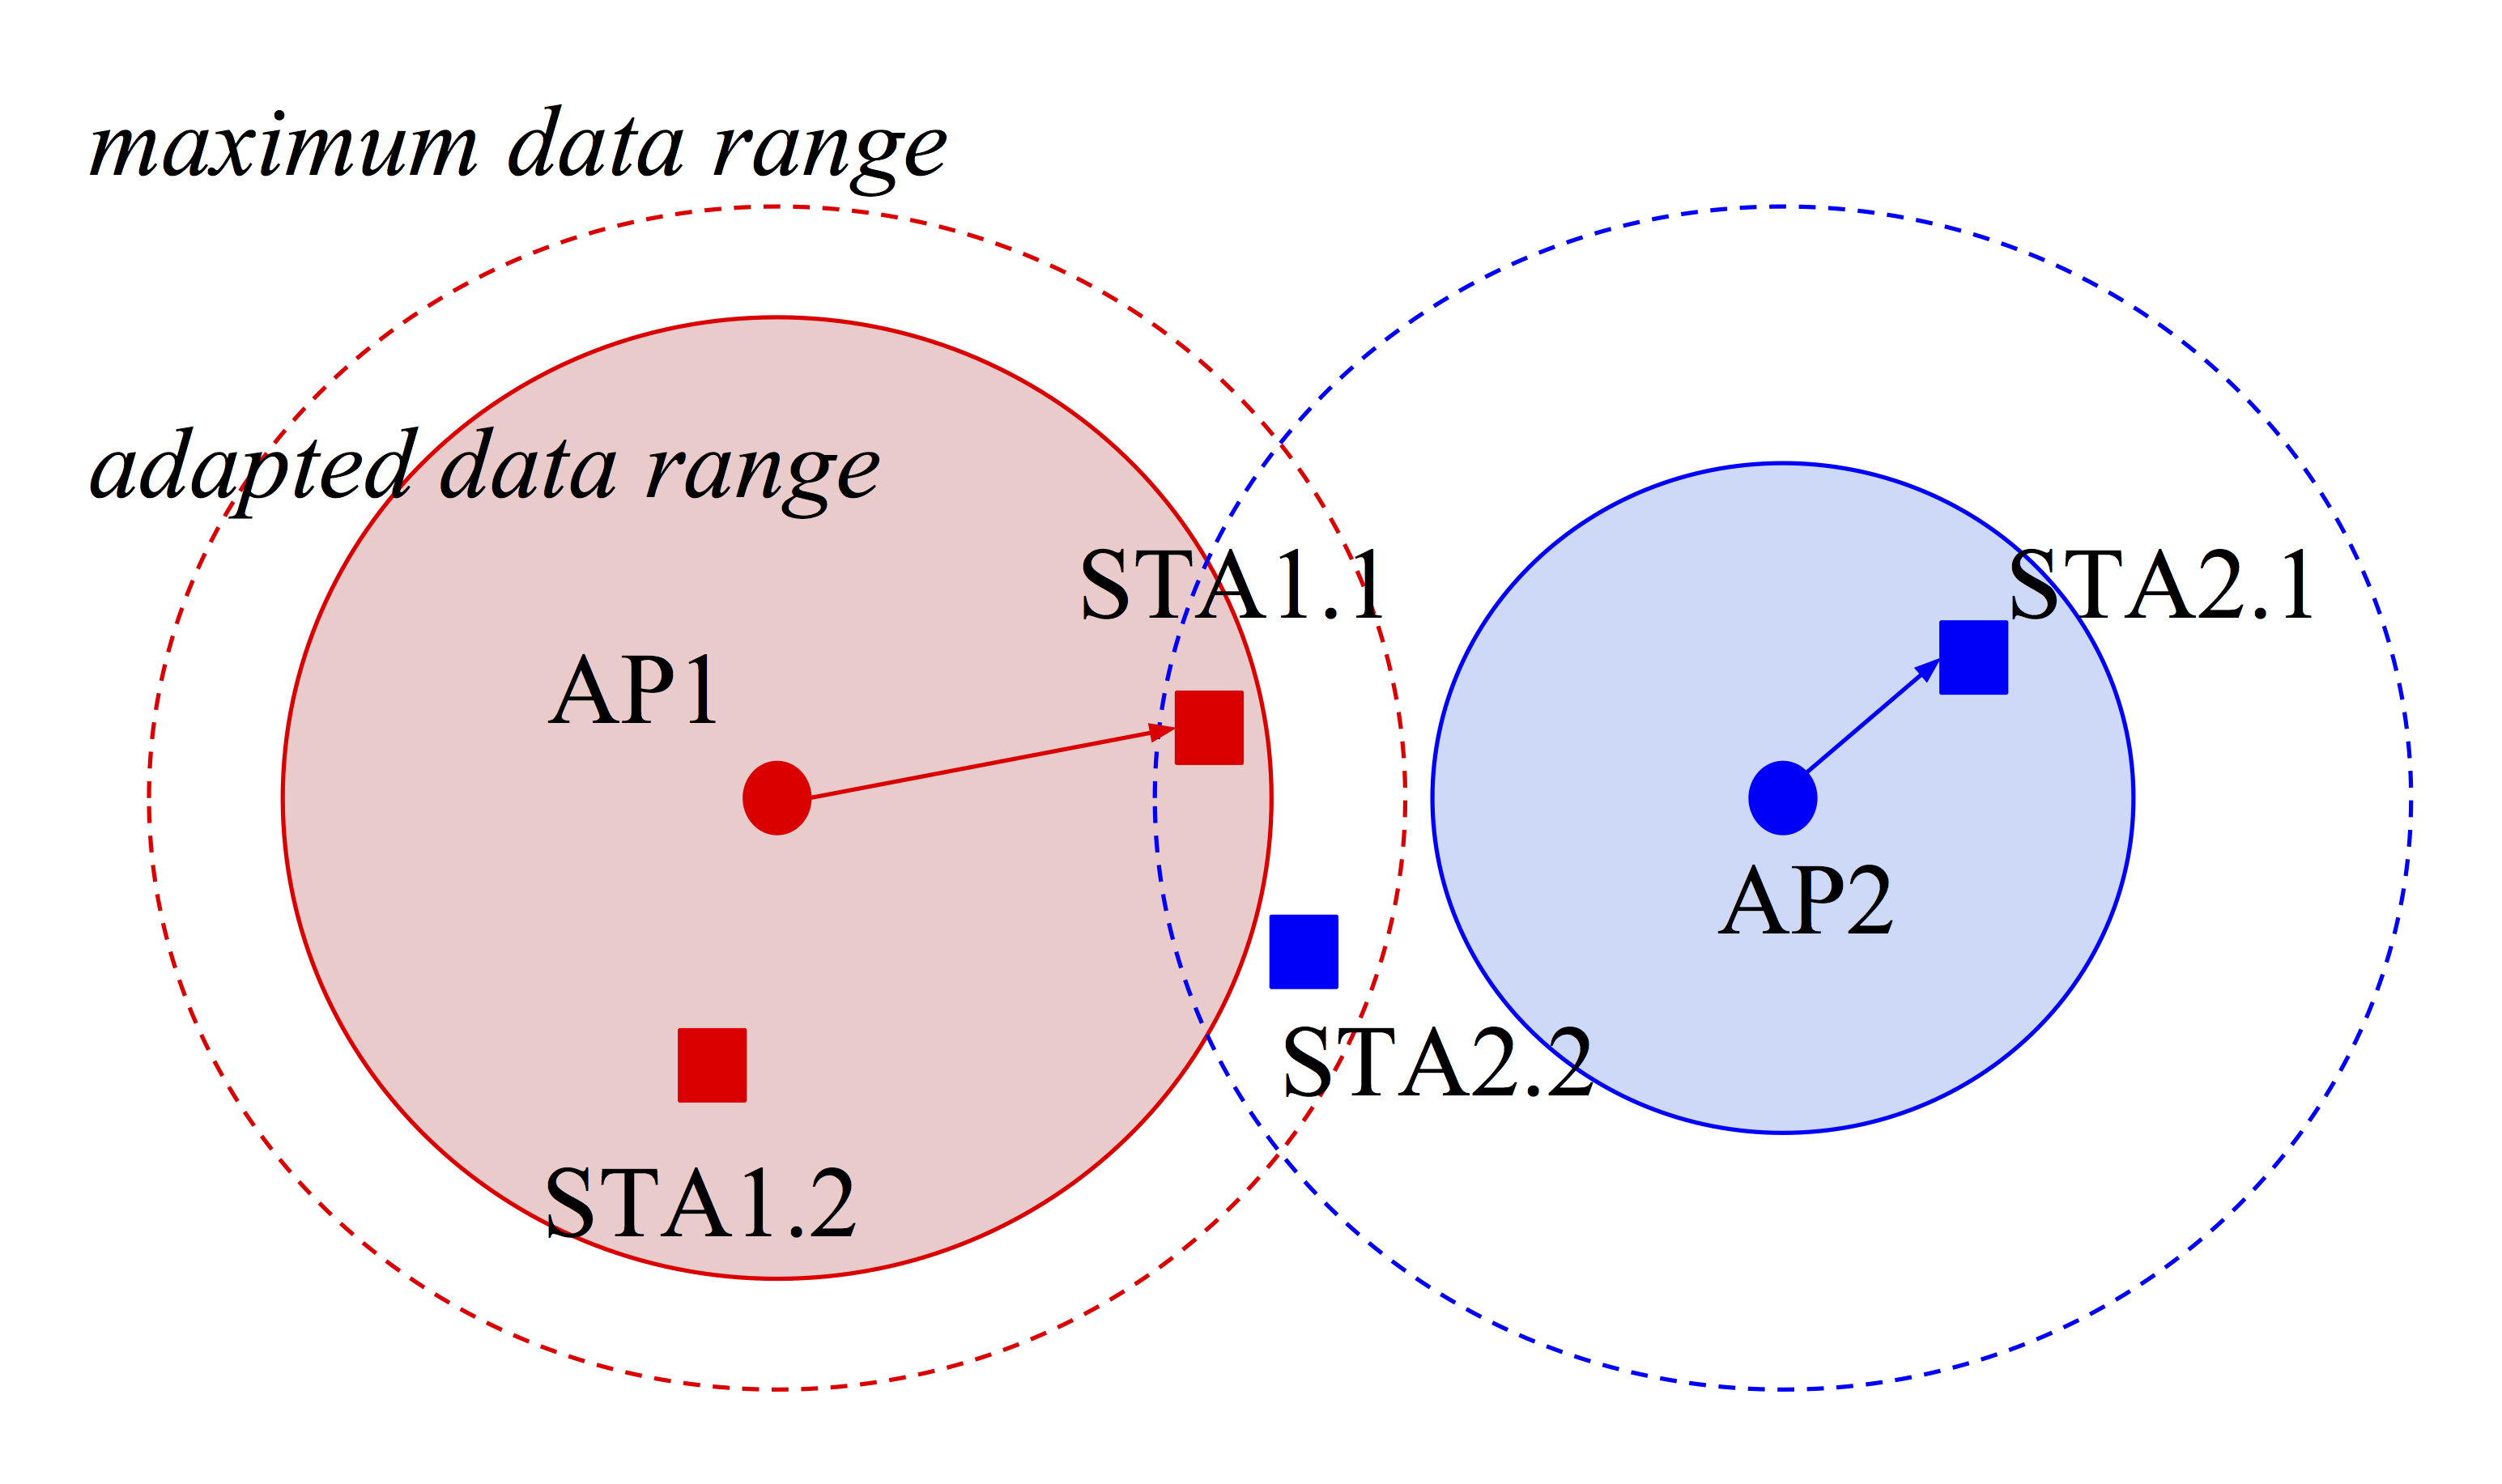
\epsfig{file=images/fcsma.png, width=11cm}
					\caption{F-CMSA operation. AP1 uses a higher transmit power to reach its farthest STA (STA1.1). At the same time, AP2 transmits to a close device (STA2.1), so that transmit power does not affect the other ongoing transmission. This scheduling is provided by a central entity.}
					\label{fig:fcsma}
				\end{figure}	
			
				Another approach that uses observations to determine the power level to be used is shown in \cite{gandarillas2014dynamic}. In it, the authors propose a decentralised system called Dynamic Transmission Power Control (DTPC), which is based on a set of triggered thresholds. Transmission power, channel occupancy and link status are the main inputs of the algorithm for modifying the transmit power. Two simulations are carried out to validate the DTCP algorithm. The first one only considers are very simple scenario in which interferences from two APs are shown to be minimised through DTPC. The second one analyses the impact of applying DTPC in two nodes, showing improvements in both energy consumption and throughput. In both cases, adjacent channels are used. The main problem is that thresholds are set empirically (based on simulations), so it may be dangerous to apply this to other scenarios different than from simulations.	Moreover, a centralised TPC mechanism is proposed in \cite{tang2014joint}. It also includes and Rate Adaptation (RA), since the current Auto-Rate Fall back (ARF) mechanisms only consider channel fading. An interesting contribution of this work is the creation of subgroups of WLANs, according to their neighbouring relationship in terms of interference. This allows defining independent power differences between devices in the same group. This power difference is useful to avoid asymmetric links. The main drawback of this work is that graphs can become very large, and that using the channel as a decision parameter is not strong enough to determine a relationship between two nodes. As a result, many nodes in the same group may lack of mutual interference. Similarly, the authors in \cite{elbatt2000power} aim to solve the energy saving problem in ad-hoc WNs by using a protocol that dynamically adjusts the power level, so that throughput is maximised. The core idea is to create clusters, so that transmit power can be adjusted accordingly. Then, a minimum power routing scheme is provided to find the shortest path in terms of power consumption. Finally, we find a different TPC approach that is also worth to mention (\cite{ebert2000energy}), since their authors show a strong relationship between the transmit power and the packets size at reducing energy consumption in WLANs. In particular, they adjust the transmit power according to the packet size, based on prior experiments. Furthermore, they show that the energy used to transmit one payload bit in a long run is given by:
				\begin{equation}
				E_{bit_{res}} = \frac{\sum_{i=1}^N P_{tx,i} \cdot B_{all,i}}{B_{succ}} \cdot T_{bit},
				\nonumber
				\end{equation}
				where N is the number of power levels, $P_{tx,i}$ is the transmit power level $i$, $B_{all,i}$ is the packet size (including headers), $B_{succ}$ is the number of successfully received bits, and $T_{bit}$ is a bit time. 
				
				The energy consumption issue is almost approached in the context of wireless ad-hoc networks, due to the trade-off them present. On the first hand, increasing the power level increases the transmission range, but it may generate interferences that lead into collisions or starvation. On the other hand, using a low power level allows reducing the interference, but a higher number of hops may be required for a packet transmission. As a final remark, we emphasise the importance of providing a solution that properly works in case of coexisting with legacy devices. In \cite{broustis2010measurement}, it is argued that using TPC in such environments can be detrimental to the aggregate performance.
			
				Table \ref{tbl:tpc} summarises the most important reviewed works on transmit power adaptation in wireless networks.
				\begin{table}[t!]
					\centering
					\resizebox{\textwidth}{!}{\begin{tabular}{|c|l|c|l|l|}
							\hline
							\multicolumn{1}{|c|}{\textbf{Work}} & \multicolumn{1}{c|}{\textbf{Presented Approach}} & \textbf{\begin{tabular}[c]{@{}c@{}}Centralised/\\ Decentralised\end{tabular}} & \multicolumn{1}{c|}{\textbf{Positive Aspects}} & \multicolumn{1}{c|}{\textbf{Negative Aspects}} \\ \hline
							\cite{oteri2013advanced} & \begin{tabular}[c]{@{}l@{}}Minimises transmit power while \\ preserving the maximal rate to\\ minimise interference\end{tabular} &  Both & \begin{tabular}[c]{@{}l@{}}  Decentralised approach: \\$\bullet$ Introduces IIR filters to  \\ adjust TPC \\Centralised approach:  \\$\bullet$ Introduces the interesting  \\concept of F-CSMA \end{tabular} & \begin{tabular}[c]{@{}l@{}}Decentralised approach:\\$\bullet$ Depends on rate adaptation \\ $\bullet$ Only applies to dense scenarios\\ $\bullet$ May generate asymmetric links \\ $\bullet$ Heuristic parameters assignment \\is done \\ Centralised approach: \\$\bullet$ Infeasible in uncoordinated scenarios\\\end{tabular} \\ \hline
							\cite{lei2015performance} & \begin{tabular}[c]{@{}l@{}}Presents a modification of\\ RTS/CTS that introduces\\ several NAV timers, so that\\ adjusting transmit power \\ does not increase the number \\of collisions\end{tabular} & Decentralised & \begin{tabular}[c]{@{}l@{}}$\bullet$  Provides fairness \\ $\bullet$ Improves the network \\ throughput \end{tabular} & \begin{tabular}[c]{@{}l@{}}$\bullet$ Only useful at few specific cases.\\ $\bullet$ Lack of evidences in realistic scenarios.\end{tabular} \\ \hline
							\cite{gandarillas2014dynamic} & \begin{tabular}[c]{@{}l@{}}A real-time mechanism based \\on triggered thresholds is \\provided to modify the \\  transmit power according\\ to the link status and the \\ channel occupancy\end{tabular} & \multicolumn{1}{l|}{Decentralised} & \begin{tabular}[c]{@{}l@{}}$\bullet$  No extra signalling is \\ required \end{tabular} & \begin{tabular}[c]{@{}l@{}} $\bullet$ Thresholds are set empirically\\ $\bullet$ Lacks of applicability in real scenarios\end{tabular} \\ \hline
							\cite{tang2014joint} & \begin{tabular}[c]{@{}l@{}}Adjusts transmit power together \\ with the data rate\end{tabular} & Centralised & \begin{tabular}[c]{@{}l@{}}$\bullet$ A clustering approach is \\provided in order to avoid \\ link asynchronies\end{tabular} & \begin{tabular}[c]{@{}l@{}}$\bullet$ The clustering algorithm can lead to \\ inefficient and large graphs, specially\\ in dense environments\\ $\bullet$ The cost of centralisation is not studied\\ $\bullet$ Coexistence with legacy devices is not\\ considered\end{tabular} \\ \hline						
					\end{tabular}}
					\caption{State-of-the-Art on Transmission Power Control}
					\label{tbl:tpc}
				\end{table}		
			 	
			 	As a final remark, it is worth to mention that TPC does not necessarily imply an energy saving, but the opposite. For instance, a high transmit power would be required to enhance the performance of an isolated network in which the AP is far enough from the STA.								
							
		%%%%%%%%%%%%%%%%%%%%%%%%%%%%%%%%%%%%%%%
		% SoA CST										         %%%%%%%%%%%%%
		%%%%%%%%%%%%%%%%%%%%%%%%%%%%%%%%%%%%%%%						
		\section{Carrier Sense Threshold Adjustment}
		\label{section:cca}
			In addition to frequency allocation and power control mechanisms, CST adjustment is key to improve the spatial reuse. By tuning the sensitivity at the receiver, it is possible to increase the number of parallel transmissions, thus maximising the aggregate throughput. In \cite{jamil2014improving}, the authors explore the possibilities to improve the capacity in IEEE 802.11 WLANs by modifying the CST. To do so, they present a typical OBSS deployment (Figure \ref{fig:jamil_2014_1}) for studying the network performance for different CCA thresholds. An interesting pattern is shown regarding the CST and aggregate throughput relationship (Figure \ref{fig:jamil_2014_2}). Moreover, the presence of legacy devices is shown to negatively affect to the overall performance.
			\begin{figure}[t!]
				\centering
				\begin{subfigure}[b]{0.375\textwidth}
					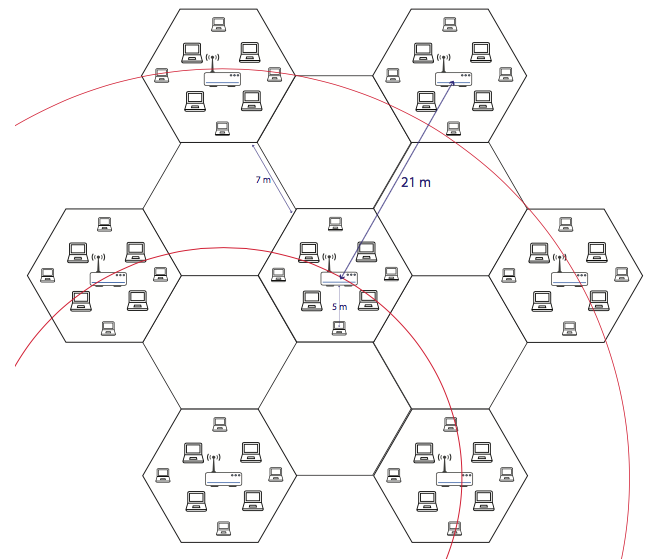
\includegraphics[width=\textwidth]{images/jamil2014_1}
					\caption{Network topology}
					\label{fig:jamil_2014_1}
				\end{subfigure}
				\begin{subfigure}[b]{0.425\textwidth}
					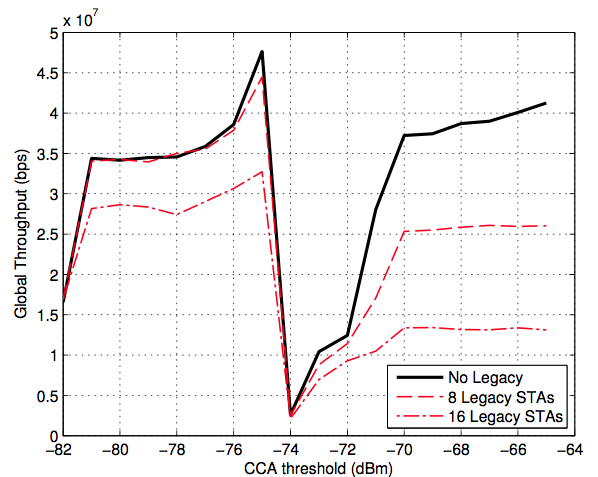
\includegraphics[width=\textwidth]{images/jamil2014_2}
					\caption{Agg. throughput vs CST value}
					\label{fig:jamil_2014_2}
				\end{subfigure}		
				\caption{IEEE 802.11ax Residential scenario}
				\label{fig:jamil_2014}
			\end{figure}		
		
			As for TPC, the TGax also introduces several limitations for adjusting the CST \cite{tgax2016draft}, so that minimum and maximum allowed sensitivity levels ($\text{OBSS\_PD}_{min}$ and $\text{OBSS\_PD}_{max}$) are determined to be -82 dBm and -62 dBm, respectively. With that, a STA can dynamically select a sensitivity level ($\text{OBSS\_PD}_{level}$) during its operation under Spatial Reuse (RS) mode, which is bounded by the aforementioned minimum and maximum levels:			
			\begin{equation}
				\resizebox{1\hsize}{!}{$\text{OBSS\_PD}_{level} \leq max\Big(\text{OBSS\_PD}_{min}, min\big(\text{OBSS\_PD}_{max}, \text{OBSS\_PD}_{min} + (\text{TX\_PWR}_{ref}-\text{TX\_PWR})\big)\Big),$
				\nonumber}				
			\end{equation}
			where $\text{TX\_PWR}$ is the STA's transmission power in dBm at the antenna connector, and $\text{TX\_PWR}_{ref}$ is set to 21 or 25 dBm according to the device capabilities\footnote{$\text{TX\_PWR}_{ref} = 21 dBm$ for non-AP STAs and for an AP with the Highest Number of Spatial Streams (NSS) Supported M1 subfield in the Tx Rx HE MCS Support field of its HE Capabilities element field equal to or less than 1. $\text{TX\_PWR}_{ref} = 25 dBm$ for an AP with the Highest NSS Supported M1 subfield in the Tx Rx HE MCS Support field of its HE Capabilities element field equal to or greater than 2.}. The obtained $\text{OBSS\_PD}_{level}$ varies for each channel width used, as shown in Table \ref{tbl:sensitivity_channel_width}.
			\begin{table}[h!]
				\centering
				\begin{tabular}{|c|l|}
					\hline
					\textbf{Channel width} & \multicolumn{1}{c|}{\textbf{$\text{OBSS\_PD}_{level}$}} \\ \hline
					40 MHz                 & $\text{OBSS\_PD}_{level}$ + 3 dB                        \\ \hline
					80 MHz                 & $\text{OBSS\_PD}_{level}$ + 6 dB                        \\ \hline
					160 MHz or 80+80 MHz   & $\text{OBSS\_PD}_{level}$ + 9 dB                        \\ \hline
				\end{tabular}
				\caption{IEEE 802.11ax specification for the sensitivity per channel width}
				\label{tbl:sensitivity_channel_width}
			\end{table}			
		
			\subsection{Dynamic Sensitivity Threshold}
			\label{section:dsc}		
				In addition to previous work related to CST adjustment (further described in Section \ref{section:other_cst}), the most important emerging approach for IEEE 802.11 WLANs is the Dynamic Sensitivity Control (DSC) algorithm, which has been proposed by the TGax \cite{smith2015dynamic}. The DSC algorithm aims to distributively find an appropriate level of CST in each non-AP station of a WLAN, in order to maximise the number of parallel transmissions and, thus the aggregate throughput. DSC periodically adjusts the CST of a wireless device given the information retrieved from Received Signal Strength Indicator (RSSI) measurements. The operation mode of DSC is graphically represented in Figure \ref{fig:dsc_flowchart}.				
				\begin{figure}[t!]
					\centering
					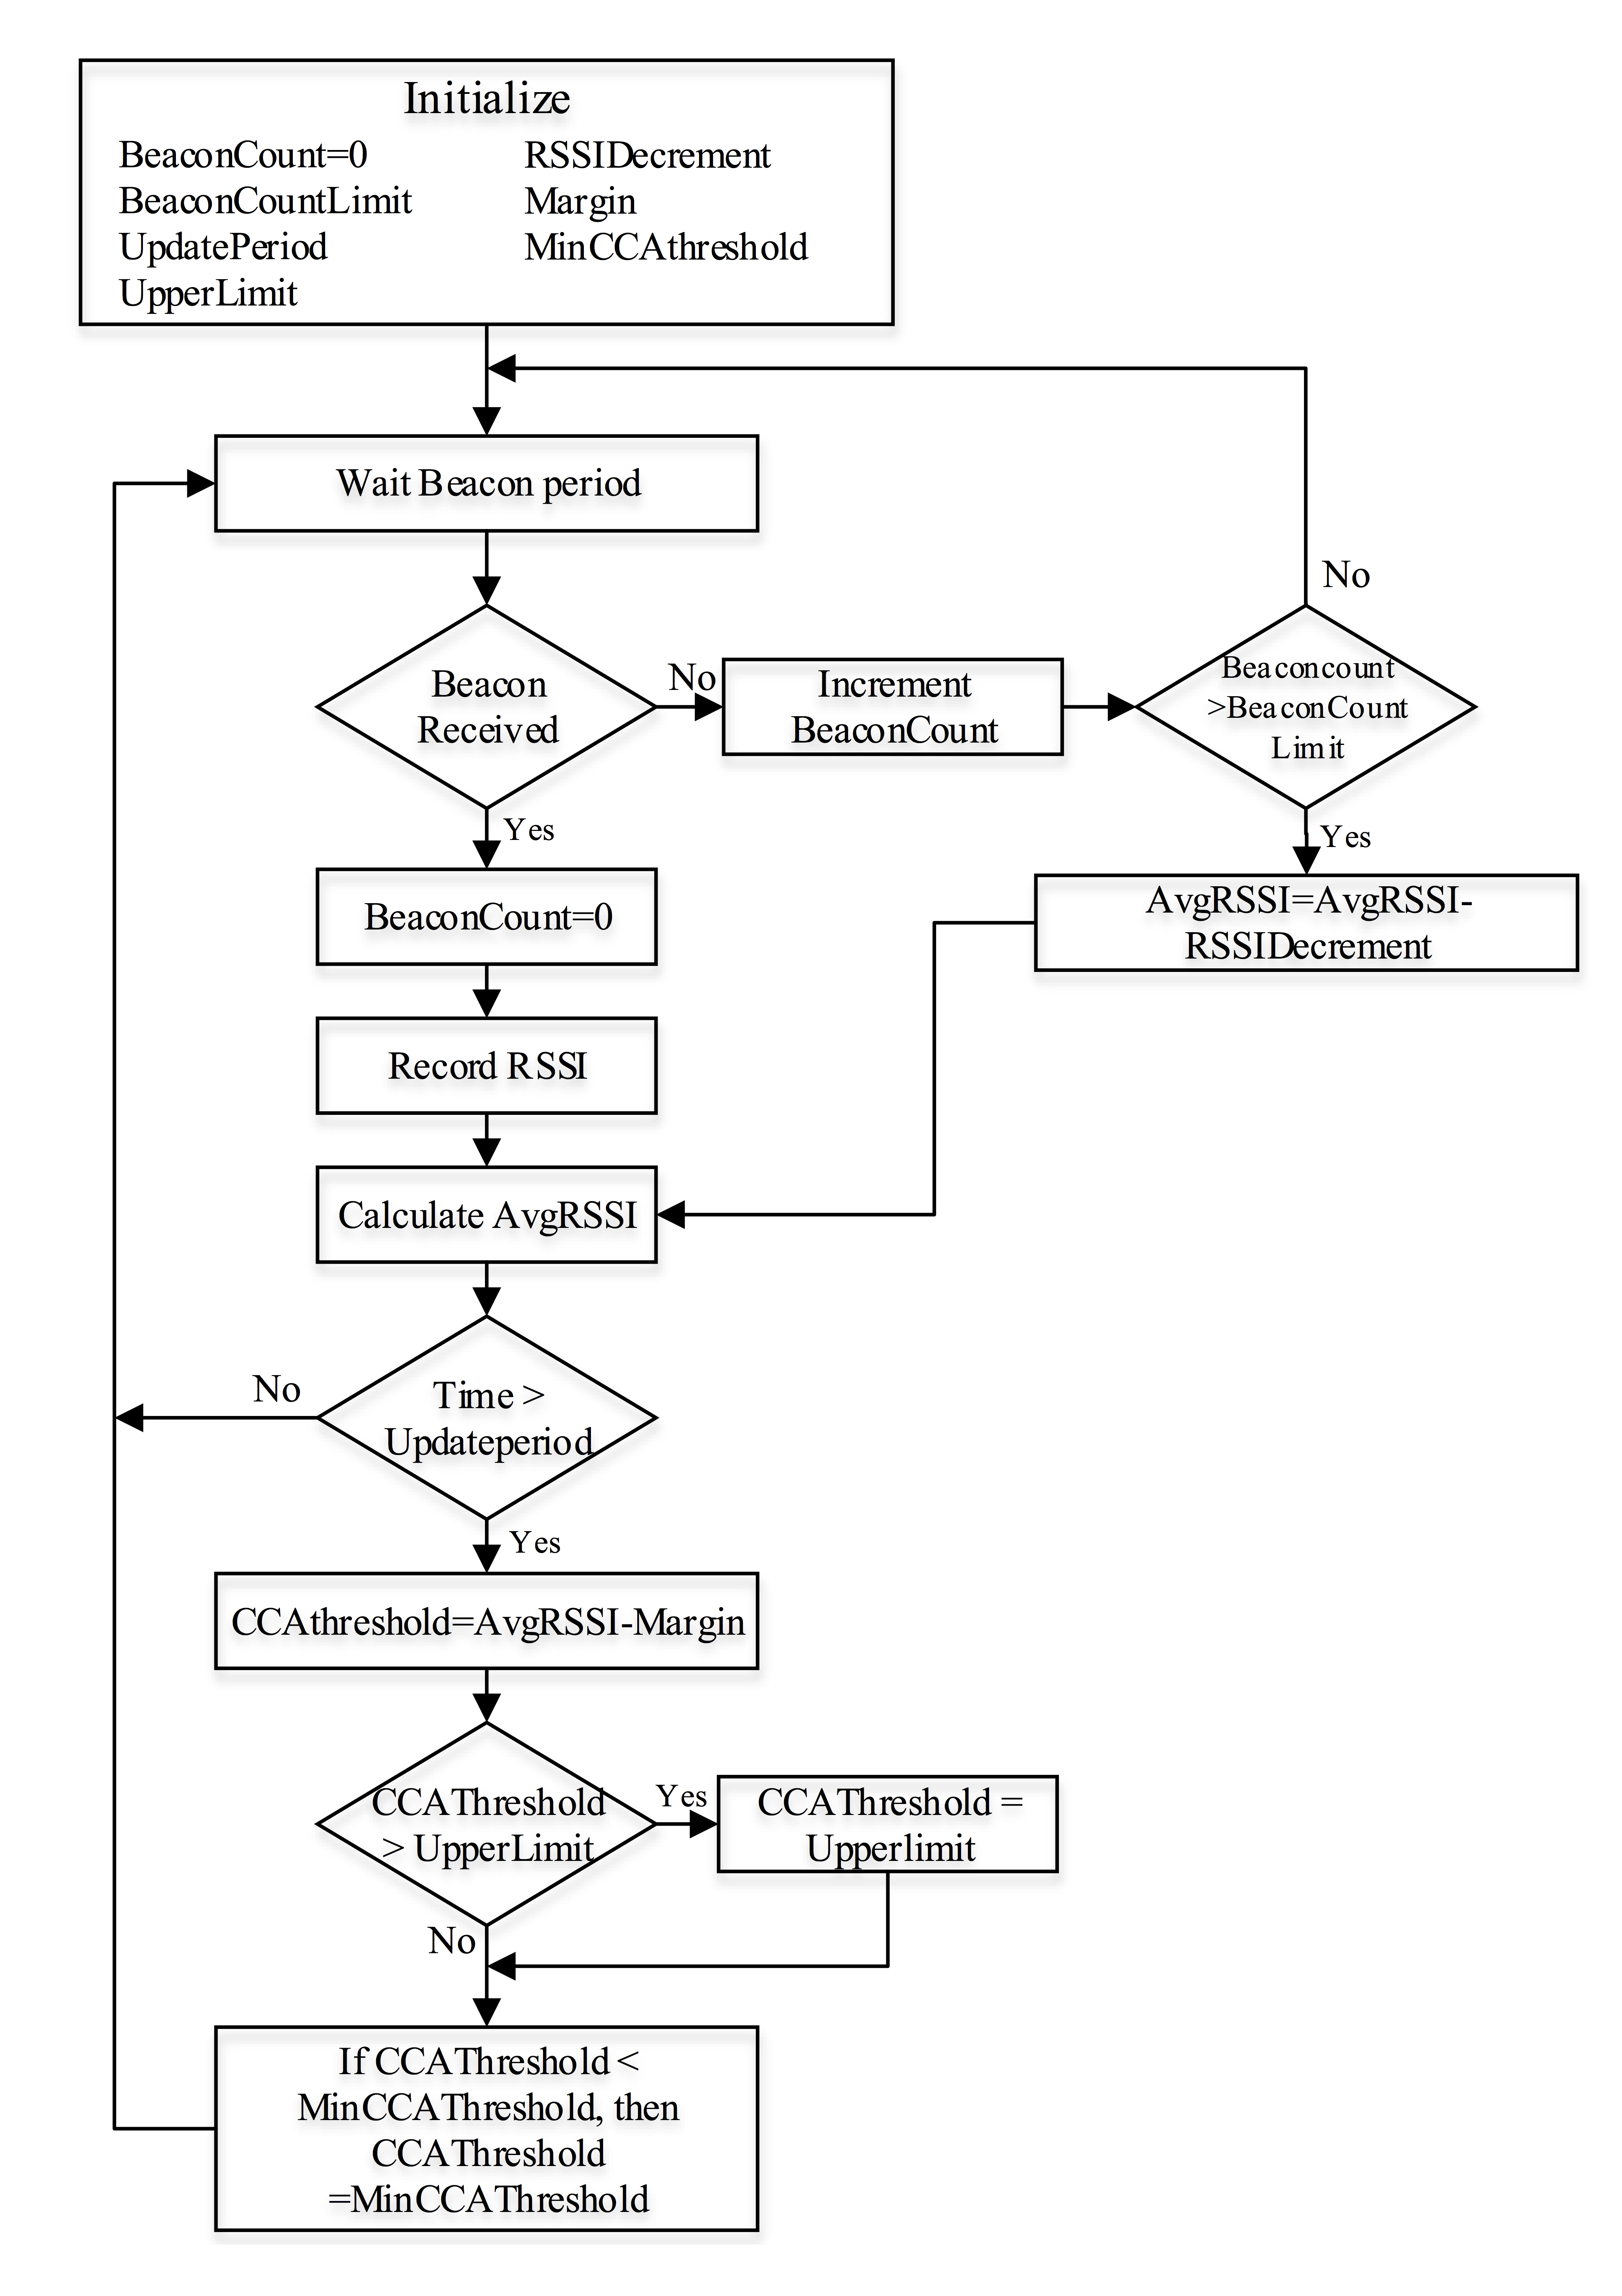
\epsfig{file=images/DSC.png, width=9cm}
					\caption{Dynamic Sensitivity Control operational mode. Image retrieved from \cite{afaqui2015evaluation}.}
					\label{fig:dsc_flowchart}
				\end{figure}
			
				In DSC, a station accumulates the Received Signal Strength Indication (RSSI) of  each  sensed  beacon until the \textit{UpdatePeriod} is reached. An average of the RSSI (\textit{AvgRSSI}) is maintained for adjusting the CST later. In parallel, it is counted the number of beacons missed during an \textit{UpdatePeriod}. At each Beacon Interval (BI) the STA compares the number of lost beacons (\textit{BeaconCount}) with a maximum threshold (i.e., \textit{BeaconCountLimit}). In case \textit{BeaconCount} is greater than \textit{BeaconCountLimit}, the average RSSI is decreased by a default value (\textit{RSSIDecrement}) with the aim of decreasing the CST and, thus listen further away to receive more beacons. Finally, after the \textit{UpdatePeriod} is reached, it is computed the new CST value between the \textit{LowerLimit} and \textit{UpperLimit} boundaries. The CST is computed as \textit{AvgRSSI} minus a margin, which is a positive number (typically from 5 to 25). An evaluation of the DSC algorithm is provided in \cite{afaqui2015evaluation}, which applies to non-AP stations in the residential scenario introduced by the TGax. On the one hand, it is shown that the overall throughput can be increased up to a 20\% with respect to legacy networks if using DSC. On the other hand, the application of DSC at uncoordinated WNs may generate a significant increase in the number of hidden nodes, which can potentially harm the overall throughput due to collisions. In fact, the increase in hidden nodes is measured to be the 60\% in the best of the cases, and the 160\% in the worst situation. Best results are obtained by using smart channel selection and fixed modulation coding scheme, while the worst results are obtained by using randomising both parameters. DSC is also evaluated in \cite{zhong2016promise}, where the Indoor Small BSSs Scenario is used for simulations. In this case, setting a low margin is substantially harmful for the overall throughput due to a very high number of collisions. Moreover, for very far distances between APs, a fixed CST behaves similarly than for using well-performing margins for DSC. In terms of fairness, the lowest margin also provides the best results (specially in the densest case). Similar results are provided in \cite{selinis2016evaluation, kulkarni2015taming} for other scenarios. While the former shows DSC performance in large-scale scenarios, the latter defends that the magnitude of the gains depends on the topology, the node distribution around the AP, the distance between overlapping cells, and the presence of cell-edge nodes. 
				
				 Without adding any kind of signalling, DSC allows enhancing the overall throughput by increasing the number of parallel transmission. However, it potentially increases the probability of collisions by hidden-node, which may be counter productive if the effects of packet losses result into worse throughput performance. Furthermore, it may generate fairness issues, since nodes with an advantageous geographical position may have more chances for accessing the channel. Figure \ref{fig:dsc_problems} shows the fairness issue in a scenario in which DSC is applied.
				\begin{figure}[h!]
					\centering
					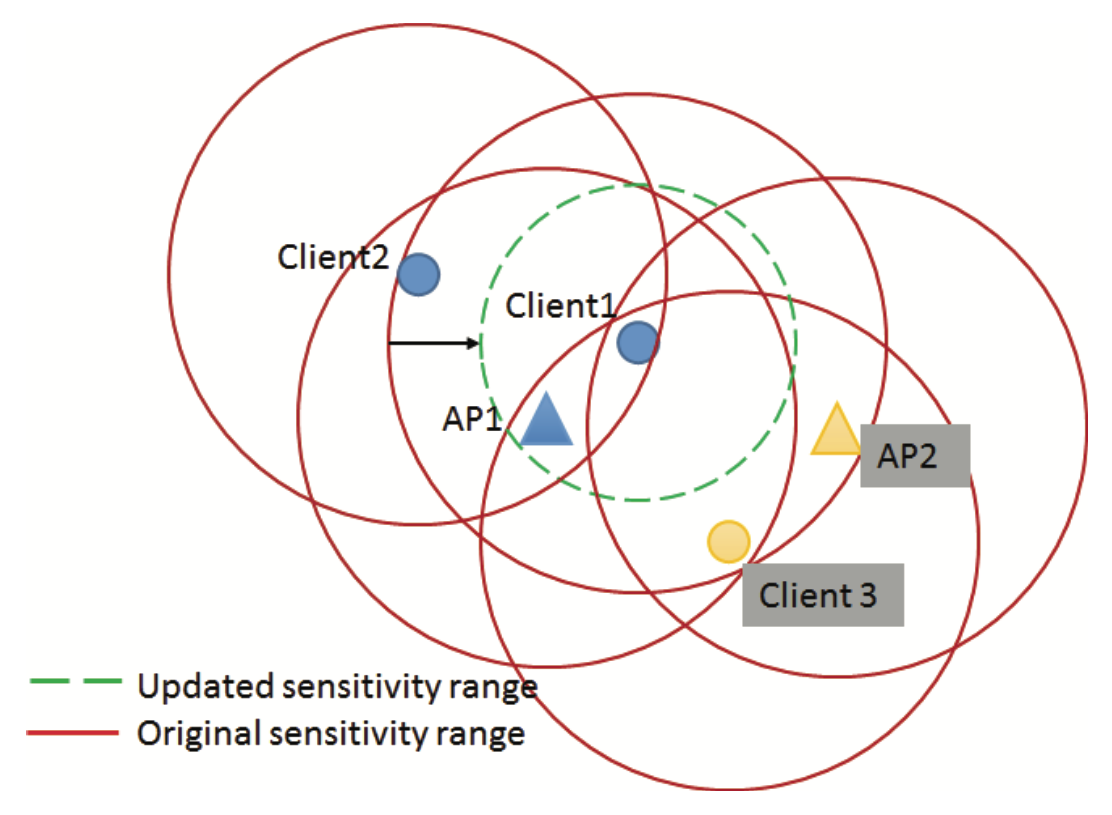
\epsfig{file=images/dsc_problems.png, width=9cm}
					\caption{DSC Fairness Issues. Client2 should have Client1 to suspend its transmission, but DSC modifies its CST in order to dismiss Client2. Image retrieved from \cite{zhong2016promise}.}
					\label{fig:dsc_problems}
				\end{figure}
					
				Further extensions of DSC have been already provided. The first one (so called DSC-AP) can be found in \cite{afaqui2016dynamic}, which intends to cover both UL and DL situations by also adjusting CST on the APs. This work is motivated by the fact that the initial DSC approach does consider the starvation problem in APs during DL transmissions. Similarly to DSC, in DSC-AP the AP records the RSSI of the received frames (either data packets or ACKs) during a period called \textit{UpdatePeriod}. The collected frames come from both associated stations and neighbouring APs. With the RSSI's information, a moving maximum RSSI ($max\mathrm{RSSI}$) is maintained for the frames received from other APs, in order to know which is the most interfering coexistent WLAN. In addition, the minimum RSSI ($min\mathrm{RSSI}$) is maintained for the frames received from the STAs within the WLAN, so that the AP can detect the farthest STA (in fact, the STA from which the AP receives the poorest signal). When the \textit{UpdatePeriod} is reached, a new CST between specific boundaries (\textit{LowerLimit} and \textit{UpperLimit}) is computed as:
				\begin{equation}
					\mathrm{CST}_{AP} = min(max(min\mathrm{RSSI}, max\mathrm{RSSI})- \text{margin}, min\mathrm{RSSI}),
					\nonumber
				\end{equation}
				where \textit{margin} is a value determined to be between 18 and 25 dB for indoor scenarios in which the path-loss factor ($\alpha$) is 0.3. The DSC-AP algorithm is shown to improve a 32\% the overall throughput with respect to legacy IEEE 802.11 performance. In addition, fairness is increased up to a 16\% because of the reduction of exposed nodes, which supposes noticing less starvation situations. The derived problems of using DSC-AP are also related to the increase of hidden nodes and collisions probability. But again, for the particular presented scenario, the obtained throughput is better despite the significant increase of the Frame Error Rate (FER).	To further improve the hidden nodes issues generated by DSC, another contribution of Afaqui et al. on sensitivity adjustment (\cite{afaqui2016rtscts}) attempts to combine DSC with RTS/CTS activation in stations. In particular, three approaches for enabling RTS/CTS in a given station are shown in combination with DSC. As for previous work, the IEEE 802.11ax Residential scenario is used for simulations. The maximum improvement shows an increase of approximately 55\% in the overall throughput with respect to legacy IEEE 802.11 performance. In addition, the FER is reduced almost a 40\% and fairness is increased in a 30\%. The fact of enabling RTS/CTS dynamically allows reducing the effects of hidden nodes in terms of collisions without adding too much overhead due to RTS/CTS transmissions, as well as it is only used in nodes that really require it. In opposite, many communication overhead is added to decide which nodes must use RTS/CTS, which has not been quantified for showing the resulting throughput when using this approach.
			
			\subsection{Previous work in CST adjustment}
			\label{section:other_cst}
				Regarding previous work that aims to adjust the CST for spatial reuse enhancement in WNs, we first focus on the work in \cite{thorpe2009ieee802, thorpe2011ieee802}, where single AP systems use the IEEE 802.11k standard \cite{ieee2002ieee} for CST adaptation. The 802.11k defines a set of mechanisms for exchanging information between nodes in a BSS, regarding the radio channel. Thus, by implementing this standard, a node measures MAC and PHY conditions, in order to share it. In \cite{thorpe2009ieee802}, an algorithm called K-APCS uses the information exchanged through the 802.11k standard to adjust the CST in real time. Motivated by the unfairness provided by K-APCS, the authors extended their work in \cite{thorpe2011ieee802}, where K-APCS2 is presented. In this case, the information exchanged by nodes is used to devise problem nodes, which are targeted by the CST optimisation algorithm. A similar approach is found in \cite{zhu2006adaptive}, which uses the Packet Error Rate (PER) locally to tune the CST in a given node. 
				
				A step further to CST adaptation is found in \cite{afifi2016throughput}, which faces the trade-off between increasing the network throughput and preserving the fairness in presence of legacy devices (i.e., devices that do not apply CST adjustment). To that purpose, the authors propose a centralised approach, Centralized Fairness Mechanism (CFM), that allow STAs to adapt their CCA according to network conditions. Thus, the AP implementing CFM, dynamically switches between the CCA adaptation phase, and the fixed phase. For the former, a new field is proposed to be included in beacons, which indicates if CCA adjustment is allowed or not. The decision of going into the CCA adaptation state is made by the AP according to the associated STAs, so that throughput can be maximised when no legacy devices are present.
				
				In addition to the aforementioned works in CST adjustment, we find other Multiple AP (MAP) collaborative approaches. \cite{hua2009cooperative, hua2009distributed} propose a distributed mechanism for CST adjustment in MAP WLANs. To achieve a jointly operation, a central unit is required, which is only feasible at fully controlled environments in which the service provider has access to the entire network.
			
			To recap the content shown in this Section, a summary of the most remarkable work in CST adjustment in shown in Table \ref{tbl:cca}.			
			\begin{table}[h!]
				\centering
				\resizebox{\textwidth}{!}{\begin{tabular}{|c|l|c|l|l|}				
					\hline
					\multicolumn{1}{|c|}{\textbf{Work}} & \multicolumn{1}{c|}{\textbf{Presented Approach}} & \textbf{\begin{tabular}[c]{@{}c@{}}Centralised/\\ Decentralised\end{tabular}} & \multicolumn{1}{c|}{\textbf{Positive Aspects}} & \multicolumn{1}{c|}{\textbf{Negative Aspects}} \\ \hline
					\cite{smith2015dynamic} & \begin{tabular}[c]{@{}l@{}}Dynamic Sensitivity Control\\ to increase the number \\of parallel transmissions\end{tabular} & Decentralised & \begin{tabular}[c]{@{}l@{}}$\bullet$ Fully decentralised \\(no signalling required) \\ $\bullet$ Easy for implementation\\ $\bullet$ Proposed by the TGax\end{tabular}  &  \begin{tabular}[c]{@{}l@{}} $\bullet$ It potentially increases \\ the number of hidden nodes \\ $\bullet$ Setting the \textit{margin} parameter \\is not clear and does not suit \\different scenarios\end{tabular}\\ \hline
					\cite{thorpe2009ieee802, thorpe2011ieee802} &  \begin{tabular}[c]{@{}l@{}} Distributed adaptive CST \\ through IEEE 802.11k\end{tabular} & Decentralised & \begin{tabular}[c]{@{}l@{}} $\bullet$ Easy to implement\\ $\bullet$ Communication overhead\\ is not an issue for the overall \\performance\end{tabular} &  \begin{tabular}[c]{@{}l@{}} $\bullet$ Lack of scalability\\ to other scenarios\\ $\bullet$ Unfairness approach\end{tabular}\\ \hline
					\cite{afifi2016throughput} &
					\begin{tabular}[c]{@{}l@{}} Centralised adaptive CST in \\presence of legacy devices \end{tabular} & Centralised  & \begin{tabular}[c]{@{}l@{}} $\bullet$ Provides effective results\\ $\bullet$ Fair approach\end{tabular} &  \begin{tabular}[c]{@{}l@{}} $\bullet$ Requires a central unit\\ $\bullet$ The presence of legacy \\nodes forces to use the default\\ operational mode\\ $\bullet$ Does not solve node problems\end{tabular} \\ \hline
					\cite{hua2009cooperative, hua2009distributed}  &
					 \begin{tabular}[c]{@{}l@{}} Distributed adaptive CST for \\ MAP WLANs\end{tabular} & Centralised  & \begin{tabular}[c]{@{}l@{}} $\bullet$ Provides effective results\\ $\bullet$ Fair approach\end{tabular} &  \begin{tabular}[c]{@{}l@{}} $\bullet$ Requires a central unit\\ $\bullet$ Infeasible in many scenarios\end{tabular} \\ \hline
				\end{tabular}}
				\caption{Carrier Sense Threshold Adjustment State-of-the-Art}
				\label{tbl:cca}
			\end{table}
		
		%%%%%%%%%%%%%%%%%%%%%%%%%%%%%%%%%%%%%%%
		% TPC & CCA RELATIONSHIP		            %%%%%%%%%%%%%
		%%%%%%%%%%%%%%%%%%%%%%%%%%%%%%%%%%%%%%%		
		\section{TPC and CCA Relationship}
		\label{section:tpc_cst_relationship}
			As previously seen in Sections \ref{section:tpc} and \ref{section:cca}, adjusting either the transmit power or the CST can contribute to improve spatial reuse, but presents several trade-offs. To even improve networks performance, there is a research line that argues for a relationship between the power transmitted and the sensitivity threshold, which is based on the naive principle ``to shout, you need to listen more carefully". According to \cite{thorpe2014survey}, by using free space path loss, the average Received Signal Strength (RSS) can be computed as a function of the distance between the transmitter and the receiver:		
			\begin{equation}
				RSS = \overline{RSS} \Big( \frac{\overline{d}}{d_{(tx,rx)}} \Big)^{\delta}
				\nonumber
			\end{equation}
			where RSS is the signal strength at the receiving node, $\overline{RSS}$ is the power of the signal received at the defined distance $\overline{d}$ (typically 1 meter), $d_{(tx,rx)}$ is the distance between the transmitter and the receiver, and $\delta$ is the path-loss exponent (often set between 2 and 4, according to the environment).  Thus, the reception range $D_{tx}$ and the carrier sense range $D_{cs}$ can be defined as:
			\begin{equation}
				D_{cs} = \overline{d} \Big( \frac{\overline{RSS}}{T_{cs}} \Big)^\frac{1}{\delta}, 				D_{rx} = \overline{d} \Big( \frac{\overline{RSS}}{T_{rx}} \Big)^\frac{1}{\delta}
				\nonumber
			\end{equation}
			Since the correct reception of data in a given node is subject to the RSS received (must be greater than the CST) and the SINR (must be greater than the capture effect), it is worth to compute the interference range $D_{I_{tx,rx}}$ as:					
			\begin{equation}
				D_{I_{tx,rx}} = d_{(tx,rx)} \times \alpha ^{\frac{1}{\delta}}
				\nonumber
			\end{equation}			
			where $\alpha$ is the minimum SINR required to achieve a correct decoding of the signal at the receiving node. The interference range is the greatest distance from which a node can be affected by another transmitting node. Figure \ref{fig:tx_cca_relation} shows the relationship between $D_{cs}$ and $D_{I_{tx,rx}}$ . 
			\begin{figure}[h!]
				\centering
				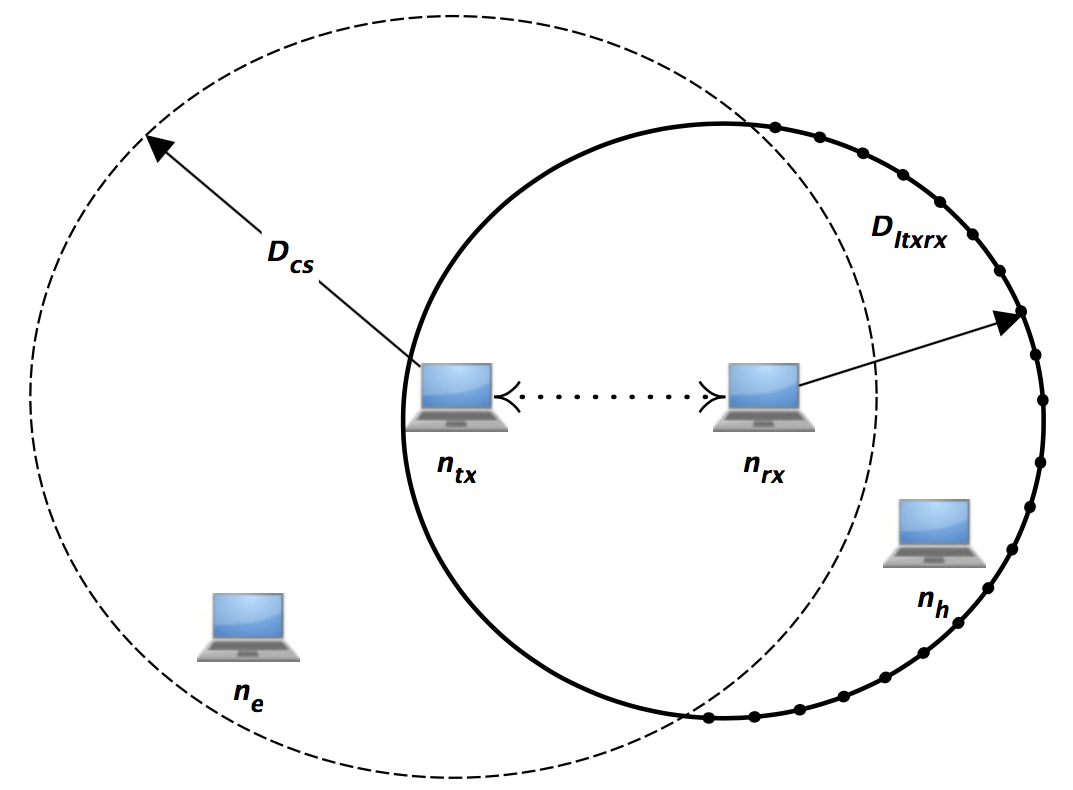
\epsfig{file=images/tx_cca_relation.png, width=9cm}
				\caption{Transmit power and CST relationship.$D_{I_{tx,rx}}$ is represented by the smaller circle with the solid line, and $D_{cs}$ is depicted by the larger circle with the broken line. Nodes $n_h$ and $n_e$ are hidden and exposed nodes, respectively. Image retrieved from \cite{thorpe2014survey}.}
				\label{fig:tx_cca_relation}
			\end{figure}	
			
			Another reason to perform CST adjustment in combination with TPC relies in the asymmetries provoked by a modification of the transmit power in an overlapping environment. The fact of creating asymmetric links generates starvation and collisions by hidden node with a higher probability, which can result into poorer performance than if using always the same configuration \cite{kawadia2005principles}. In relation to these performance anomalies, \cite{mhatre2007interference} defends that tuning TPC and CST together is a must for improving spatial reuse in WLANs. For that, it shows that links remain symmetric in a situation in which the power transmitted and the sensitivity threshold are adjusted together. Moreover, it proposes a method based on Gibbs sampling for distributively adjusting both TPC and CCA. The algorithm is tested in dense scenarios (72 APs and 288 clients), showing remarkable improvements in the average throughput (it is increased by a $290\%$) after convergence occurs. Interestingly, from results it is derived that the power transmitted per AP is inversely proportional to the sensitivity.				
			
			Many other works exploit the relationship between the transmit power and the CST to enhance fairness and throughput performance in wireless networks. In \cite{jamil2015preserving}, improving fairness is the main goal (although the overall throughput is also enhanced). To achieve that, each time a beacon is received in a STA, it is measured a parameter to adapt both CST and transmit power: $\Delta_x = Rx_p - M - PCS_{default}$, where $Rx_p$ is the power received (depends on the power transmit and the attenuation loss), $M$ is a margin (in this case it is set to 20 dB), and $PCS_{default}$ is the default minimum CST (for channels of width 20 MHz, $PCS_{default}$ is -82 dBm). Then, the difference of CST and TPC is computed from $\Delta_x$ and a given ratio
			\begin{equation}
				\Delta_{TPC} = ratio \times \Delta_x, \Delta_{CCA} = \Delta_x - \Delta_{TPC}
				\nonumber
			\end{equation}
			Finally, the TPC and the CST are modified by increasing/decreasing the obtained adaptation values ($TPC = TPC - \Delta_{TPC}$ and $CCA = CCA + \Delta_{CCA}$, respectively). The $ratio$ determines the adaptation degree of CST and TPC (setting the ratio to 0 entails only CST adaptation, while setting it to 1, only TPC). To adapt both CST and TPC, so-called Balanced TPC and PCS Adaptation (BTPA), the chosen $ratio$ is 0.5, but during the simulations it is also shown the results of adapting CST and TPC separately. The scenario consists in a cellular network composed by 7 APs that transmit data to 8 STAs each one.	The results are significant, since the average throughput is increased by a 4 factor while preserving the fairness coefficient to 1. Despite being very simple, this mechanism allows improving the spatial reuse while preserving fairness. The authors in \cite{kim2006improving} also consider the TPC and CCA relationship, but put special emphasis on the trade-off between increasing spatial reuse and decreasing individual transmission data rate. Thus, they present a decentralized algorithm that adjusts power and rate control in a node, given the interference level it perceives. It is also sought to keep the highest possible data rate, while keeping minimal the generated interference towards neighbouring WLANs. To do so, the presented approach first determines the minimum power to be used so that the receiver can properly decode the message. Then, the CST is set to the minimum value at which the incoming signal is sensed, which depends on the perceived interference. To solve the problem in which the transmitter does not know the interference level $I_{RX}$ at the receiver, the authors propose to set the CST at the transmitter as a function of the SINR. The provided adjustment function ensures that the interference at the receiver is not higher than a given threshold that depends on the power transmitted, and that the minimal data rate is sustained. The key is to restrict the transmit power based on the estimated distance between the transmitter and the interfering node. Through simulations in different scenarios (from low to high density), it is shown a significant improvement at both aggregate throughput and average saved power (up to 22\% and 50\%, respectively). As in previous works, \cite{oteri2015improved} shows the benefits of using both TPC and CCA adaptation in the context of IEEE 802.11ax WLANs. Furthermore, it provides evidences that different results may be obtained according to the scenario (due to path-loss effects in presence of walls). Finally, a rigid approach for fully controlled networks is presented in \cite{zhu2004leveraging}, where the CST to be used by devices in a mesh WN is computed as a function of the distance between nodes, and assuming that the same transmit power is used. In particular, different CST equations are provided for grid and line topologies, since the interference pattern varies. In this case, all the devices are considered to be placed symmetrically. Thus, an ideal situation is proposed for planned and interference-free deployments (e.g. a rural sensors deployment). However, this approach turns out to be unrealistic in chaotic wireless deployments.
			
			To summarise the most remarkable work in CST adjustment in combination with TPC, in Table \ref{tbl:tpc_cca} we show the key features of each work reviewed in this section.			
			\begin{table}[h!]
				\centering
				\resizebox{\textwidth}{!}{\begin{tabular}{|c|l|c|l|l|}				
						\hline
						\multicolumn{1}{|c|}{\textbf{Work}} & \multicolumn{1}{c|}{\textbf{Presented Approach}} & \textbf{\begin{tabular}[c]{@{}c@{}}Centralised/\\ Decentralised\end{tabular}} & \multicolumn{1}{c|}{\textbf{Positive Aspects}} & \multicolumn{1}{c|}{\textbf{Negative Aspects}} \\ \hline
						\cite{mhatre2007interference} & \begin{tabular}[c]{@{}l@{}} Gibbs sampler to \\adjust both TPC and CCA\end{tabular} & Decentralised & \begin{tabular}[c]{@{}l@{}}$\bullet$ Dense scenarios are\\ considered \\$\bullet$ Significant improvements\\in the average throughput\end{tabular}  &  \begin{tabular}[c]{@{}l@{}} $\bullet$ Complex implementation\end{tabular}\\ \hline						
						\cite{jamil2015preserving} & \begin{tabular}[c]{@{}l@{}} TPC and CCA adjustment\\ in WLANs to improve\\ fairness\end{tabular} & Decentralised & \begin{tabular}[c]{@{}l@{}}$\bullet$ Very simple\\$\bullet$ Significant improvements\\in the average throughput\end{tabular}  &  \begin{tabular}[c]{@{}l@{}} $\bullet$ Simulation scenarios \\are too rigid\end{tabular}\\ \hline
						\cite{kim2006improving} & \begin{tabular}[c]{@{}l@{}} TPC and CCA adjustment\\in D2D networks\end{tabular} &  Decentralised & \begin{tabular}[c]{@{}l@{}}$\bullet$ Very simple\\$\bullet$ Significant improvements\\in the average throughput\end{tabular}  &  \begin{tabular}[c]{@{}l@{}} $\bullet$ Simulation scenarios \\are too rigid\\$\bullet$ The power limitation \\ may entail performance \\issues to many scenarios\end{tabular}\\ \hline
						\cite{zhu2004leveraging} & \begin{tabular}[c]{@{}l@{}} CCA adjustment according \\to the distance between \\nodes and the transmit \\power \end{tabular} & Centralised  &  \begin{tabular}[c]{@{}l@{}} $\bullet$ Great enhancements are \\achieved\end{tabular} & \begin{tabular}[c]{@{}l@{}} $\bullet$ Only applicable to \\fully controlled networks\\ $\bullet$ Only rigid topologies\\ are allowed\\ $\bullet$ The same transmit power\\must be used by all the\\ devices\end{tabular} \\ \hline
				\end{tabular}}
				\caption{TPC and CCA Relationship State-of-the-Art}
				\label{tbl:tpc_cca}
			\end{table}
		
		%%%%%%%%%%%%%%%%%%%%%%%%%%%%%%%%%%%%%%%
		% SoA BEAMFORMING						         %%%%%%%%%%%%%
		%%%%%%%%%%%%%%%%%%%%%%%%%%%%%%%%%%%%%%%						
		\section{Beamforming}
		\label{section:beamforming}
			Beamforming \cite{van1988beamforming} is a signal processing technique for transmitting beams of energy to a given receiver. By narrowing the signal occupancy in the space, it is possible to reduce the number of contending nodes, thus enhancing spatial reuse in an overlapping wireless scenario. Furthermore, directional antennas allow reaching farther distances, which contributes to increase the range of a network. In \cite{athan2004antenna}, the usage of beamforming is shown to significantly increase the network capacity, as a result of increasing spatial reuse. The application of beamforming has been mostly applied to ad-hoc wireless networks \cite{ramanathan2001performance, spyropoulos2003capacity, yi2003capacity}, which shows great throughput enhancements by reducing the average number of hops in packet transmissions. Nevertheless, beamforming may also lead to performance issues, such as hidden or terminal problems. According to \cite{alawieh2009improving}, the following problems may be encountered:
			\begin{itemize}
				\item Deafness: occurs when a node transmits to another one that is already transmitting. As a result, the new transmission is dismissed. The deafness issue is motivated by the fact that the first transmission is not heard by the interfering node, which may also lead into a collision by hidden node. Consequences of the deafness problem in ad-hoc wireless networks are studied in \cite{choudhury2005performance}.
				\item Hidden terminal: similarly to deafness, an ongoing transmission is not sensed, so that new transmissions may lead into collisions. The hidden terminal problem for directional antennas is studied in \cite{arora2004directional}. 
				\item Exposed terminal: this problem occurs when nodes are too close and the energy beam is not accurate enough to reduce the number of contending nodes. The exposed terminal problem for directional antennas is studied in \cite{wang2005syn}.
				\item Head of line blocking: extra delays can occur in First-In-First-Out (FIFO) systems due to the exposed terminal problem. For instance, in case node A has packets for B and C, respectively, but B is in between an ongoing transmission, the fact of using FIFO prevents to transmit first to C, which appears to be ready for receiving the packet.
			\end{itemize}
			Despite of the issues arisen from the usage of directional antennas, beamforming is a promising technique that has been of particular interest in recent years. In combination with power control, directional antennas have been shown to be effective at both throughput enhancement and energy consumption saving \cite{fahmy2002ad, nasipuri2002power}.	
		
		%%%%%%%%%%%%%%%%%%%%%%%%%%%%%%%%%%%%%%%
		% RL							    							%%%%%%%%%%%%%
		%%%%%%%%%%%%%%%%%%%%%%%%%%%%%%%%%%%%%%%
		\section{Reinforcement Learning}
		\label{section:rl}				
			Reinforcement Learning frames the problem in which an agent learns by interacting with the environment (which can be dynamic), with the aim of maximising a long-term objective function. Typically, a RL problem can be modelled through a Markov Decision Process (MDP), which is defined as a tuple $\mathcal{M} = \langle \mathcal{S}, \mathcal{A}, R, T\rangle$:
			\begin{itemize}
				\item $\mathcal{S}$ is the set of possible states in which the agent can be.
				\item $\mathcal{A}$ is the set of possible actions that the agent can do.
				\item $R_{a,s}$ is the reward generated by the environment  when the agent makes an action $a \in \mathcal{A}$ when being in the state $s \in \mathcal{S}$.
				\item $T(s,a,s')$ is the probability of transitioning from state $s$ to $s'$ after doing action $a$.
			\end{itemize}
			The goal of the agent is to learn the policy that allows maximising the total reward (Figure \ref{fig:rl_scenario}). 
			\begin{figure}[h!]
				\centering
				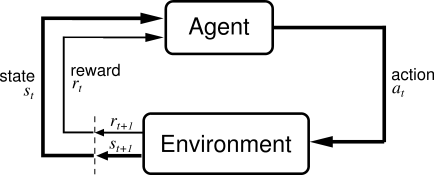
\epsfig{file=images/rl_scenario.png, width=8cm}
				\caption{Basic RL scenario. Image retrieved from \cite{sutton1998reinforcement}}
				\label{fig:rl_scenario}
			\end{figure}		
		
			Many RL problem formulations can be found according to the desired performance (long-term or short-term reward) and the data collection process (full or partial information). The most important RL problems are modelled through Markov Decision Processes (MDPs), so that the transition between states is carried out after doing actions. Value iteration methods are often used to solve MDPs, except for large-scale problems and scenarios in which full information of the model is not available. 
			Although RL problems are often categorised into Batch (learn the entire training data) and Online learning (learn progressively), in \cite{szepesvari2010algorithms} we find a nice categorisation of RL problem types and approaches, which are summarised in Figure \ref{fig:rl_types}.			
			\begin{figure}[h!]
				\centering
				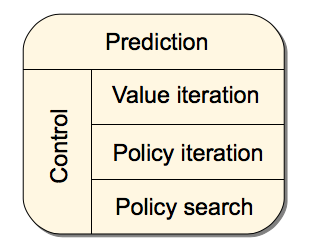
\epsfig{file=images/rl_types.png, width=5cm}
				\caption{Types of RL problems and approaches. Image retrieved from \cite{szepesvari2010algorithms}}
				\label{fig:rl_types}
			\end{figure}
					
			The first group (Prediction), considers state-dependent problems, so that the value function is estimated by the learner. In practice, prediction methods describe, after ending the learning process, the expected reward when making actions from a given state. Monte-Carlo methods \cite{robert2004monte} are the basic form of value prediction, since them estimate the average value over multiple independent simulations. However, these kind of methods often perform poorly because they do not consider the variance between experiments. In addition, the fact of starting from the same state results to be infeasible in many occasions. To solve that, Temporal difference (TD) learning was firstly introduced in \cite{sutton1988learning}. TD aims to maintain an estimate of the value in a given state by means of considering past information. For that, it includes the notion of the step-size sequence ($\alpha_t$), which are non-negative numbers that regulate the importance of past information in a given step $t$. Moreover, and to cover a large space of states (i.e., states do not fit in memory), function approximation methods are required. In this case, a feature extraction method is used to model a given state to a $d$-dimensional vector (e.g., with a polynomial function, state $x$ can be converted into $\varphi(x) = (1, x, x^2, ..., x^d-1)$).  Among function approximation methods, we find gradient descend (e.g., GTD2 and TDC), and least-squares methods (e.g., LSTD($\lambda$) and $\lambda$-LSPE).
			
			Regarding Control methods, the aim is to find a policy that maximises the reward given a set of states. To do so, we find three main approaches: 
			\begin{itemize}
				\item \textbf{Value iteration:} computes the expected utility of each state by using information of the neighbouring states. Thus, since value iteration is only interested in finding the optimal value, a single optimal policy is obtained if recursively applying the Bellman Equation.
				\item \textbf{Policy iteration:} a value function is used to model the expected return of a given action-state pair, so that the immediate reward is used in combination with the discounted value of the next state\footnote{This method is so-called \textit{bootstrapping}}). Some examples of policy iteration techniques are Q-learning, TD-learning, SARSA and QV-learning. Finally, in policy search, no value function is used, but only the parametrised policy is stored. With that, it is sought to find the optimal parameters of the policy.
				\item \textbf{Policy search:} it is mainly used in robotics, and some well-known techniques follow Episodic (e.g., Relative Entropy Policy Search, REPS) and Evolutionary strategies (e.g., Covariance Matrix Adaptation Evolution Strategy, CMA-ES).
			\end{itemize}   
			Control methods can be categorised according to the interaction that the agent maintains with the environment (see Figure \ref{fig:rl_control_types}). If the learner can actively influence the observations, we are in the context of interactive learning. Otherwise, with no interaction, the learner can just attempt to learn the model by only making observations.			
			\begin{figure}[h!]
				\centering
				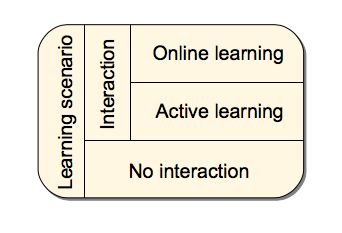
\epsfig{file=images/rl_control_types.png, width=6cm}
				\caption{Types of RL problems and approaches. Image retrieved from \cite{szepesvari2010algorithms}}
				\label{fig:rl_control_types}
			\end{figure}
			
			Since wireless networks strongly interact with the environment, from here onwards we only focus on interactive learning problems. The performance in such type of problems can be measured in many ways (sum of rewards, quantification of the mistakes done, etc.), and it is strongly related to exploration. In online learning the learner obtains data in a sequential order, so that it can be used to predict future optimal actions. Online learning is useful in case that training a entire dataset is infeasible. Moreover, it is also useful to capture dynamic environments that require self-adjusting mechanisms to perform properly over the time. State of the art algorithms in online learning are mainly given for bandits (one-state MDPs) and MDPs. Finally, in active learning, the learner can maximise the probability of finding a good policy by asking for information to the user or to a database. Unlike supervised learning, here the agent actively asks for the unknown samples. Active learning turns out to be useful when a lot of training data is available, but labelling all the samples is expensive. It is often used in the pattern recognition field (e.g. pedestrian recognition \cite{abramson2004active}).
					
			Table \ref{tbl:soa_rl} shows a set of RL families of methods, as well as their main characteristics.			
			\begin{table}[h!]
				\centering
				\begin{tabular}{|c|c|c|c|l|}
					\hline
					\textbf{Method} & \textbf{\begin{tabular}[c]{@{}c@{}}Prediction/\\ Control\end{tabular}} & \textbf{Type} & \textbf{\begin{tabular}[c]{@{}c@{}}State-\\ dependent\end{tabular}} & \multicolumn{1}{c|}{\textbf{Popular Applications}} \\ \hline
					Monte-Carlo & Prediction & Offline & Yes & Black Jack \\ \hline
					TD & Prediction & Online & Yes & TDGammon \\ \hline
					Bandits & Control & Online & No & \begin{tabular}[c]{@{}l@{}}Ranking, Resource allocation, \\ Online advertising, Routing\end{tabular} \\ \hline
					Q-learning & Control & \begin{tabular}[c]{@{}c@{}}Offline/\\ Online\end{tabular} & Yes & \begin{tabular}[c]{@{}l@{}}Inventory management, Financial\\ Trading Systems\end{tabular} \\ \hline
					SARSA & Control & Online & Yes & Gridworld, Reluctant walk \\ \hline
				\end{tabular}
				\caption{Families of RL methods}
				\label{tbl:soa_rl}
			\end{table}
					
			In general, modelling the resource allocation problem in WNs is complex, and only partial information can be obtained. Thus, we are mostly interested in model-free learning procedures, which in fact attempt to approximate value functions. In addition, the learning procedure must be carried out in an online mode, as well as there is a high variability in WNs, specially in dense environments. For that, we envision MABs to be the most suitable technique for the resource allocation problem in overlapping WNs, but we are completely open to explore other techniques.
		
			\subsection{Reinforcement Learning for improving Spatial Reuse in WNs}		
			\label{tbl:rl_to_wns}
				The current literature shows an upward trend on applying RL for solving many problems in the wireless communications fields. It is on our interest to study the cases in which RL is used to improve spatial reuse in WNs, so we first focus on \cite{nie1999q}, which uses real-time Q-learning for DCA in the context of mobile communications. To do so, states for each cell are defined as the channel selected and the available channels at time $t$. Thus, the state of a given cell depends on the states of the others. Actions are considered to be the transition between available channels, so the reward is computed as a functions that considers the channel utilisation (distance between cells is considered). Despite the discount factor is deterministically set to 0.5, the learning rate is defined for each state-action pair $(s,a)$, so that it is inversely proportional to the frequency $(s,a)$ is visited. Q-learning is implemented distributively, so that each cell is responsible for channel assignment. However, exchanging data is required to let cells know channel-status information between neighbouring base stations. The overhead of such communication is not considered. Q-learning is also used in \cite{li2009multi} for channel selection in wireless networks. In this case, considerations on multi-user environments are done, so that Multi-Agent Reinforcement Learning (MARL) is applied in a scenario composed by two devices. It is shown that using Q-learning in a such competitive environment allows doing a proper distribution of the resources (in this case, frequency channels). A further extension of the previous work applying Q-learning to the channel selection problem, is presented in \cite{bennis2010q}. In this case, self-organised femtocell networks are focused to solve both carrier and power allocation problems. The former is approach through Q-learning, while the latter is formulated using the gradient method once channel allocation is done. Contrary to previous work, the authors propose a rewarding system based on the SINR. A simulation scenario with 2 cells and 5 subcarriers is used for simulation, which compares the Q-learning performance to the random and static strategies. Again, Q-learning parameters are deterministically set to $\alpha = 0.5$ and $\gamma = 0.9$.	An extension of this is presented in \cite{bennis2011distributed}, which puts the focus on coordinated systems in order to improve the performance. A cooperative Q-learning approach is developed to show a higher performance and a faster convergence than uncoordinated systems.
					
				MABs are also becoming a popular tool in the WNs field, so in \cite{maghsudi2015joint} we find a distributed channel selection and transmit power approach for Device-to-Device (D2D) communications. The problem is modelled by considering $\mathcal{K}=\{1,...,K\}$ transmitter-receiver pairs being able to choose from $\mathcal{N}'_k$ orthogonal channels and from $\mathcal{N}''_k$ power levels. The joint action selection at time $t$ leads to the joint action profile $\textbf{I}_t$, consisting in a pair $(\textbf{I}'_t,\textbf{I}''_t)$. Thus, a reward is computed for a given joint action profile \textbf{I}. In order to show that the external regret of each user asymptotically decays with time, and that players’ actions converge into a equilibrium, two decentralized minimization strategies are presented: \textit{No-Regret Bandit Exponential-Based Weighted Average strategy} and \textit{No-Regret Bandit Follow the Perturbed Leader strategy}. For the former, each action is selected by some probability that depends on the accumulated reward of that action (the best performance an action shows, the higher will be its associated probability). The estimated reward is useful for calculating the regret of any other chosen action. Basically, the algorithm makes a D2D pair to play an arm and define a so-called parameter $\delta_{(i \rightarrow j),t}^{(k)}$ according to the experienced regret (which depends on the others' actions). With that, the probability distribution of possible actions is updated, which affects to the next action. If all players play according to NR-BEWAS, then the game converges to a correlated equilibria. In the NR-BFPLS case, the action with minimum regret is chosen, but a random perturbation is added to avoid falling into a deterministic setting. Similarly to the previous approach, actions are chosen according to the current probability distribution, which is being updated at each iteration. In this case, the reward is computed by including a perturbation, which is a two-sided exponential distribution. Simulations are carried out for two transmitter-receiver pairs that share two orthogonal channels. By using the two abovementioned action selection strategies, the optimal configuration is rapidly achieved by both users (approximately with 500 iterations for the NR-BFPLS strategy). Further simulations are done for a wireless network consisting in five transmitted-receiver pairs competing for three orthogonal channels with two possible power levels. The obtained reward for each of the approaches is shown to converge rapidly to the optimal. Furthermore, in \cite{maghsudi2015channel},  Maghsudi and Sta{\'n}czak also approach the D2D channel selection problem through Bandits, but in this case it is included a calibrated predictor (referred in the work as \textit{forecaster}) to infer the behaviour of the other devices in order to counter act their actions. At each agent, the information of the forecaster is used to choose the action with highest reward with a certain probability, while the rest of the times a random action is selected. Henceforth, assuming that all the networks use a strategy $\mathcal{X}$, fast convergence is ensured. The experimental part consists in two D2D users that must share two orthogonal channels, which shows that both users end up knowing the behaviour of the other. Thus, channel resources are optimally distributed in a very few time through a fully decentralised algorithm that does not require any kind of coordination.
			
				Finally, \cite{jamil2016novel} presents a centralized solution to adapt the transmission power and the carrier sense threshold of all the devices in a wireless network, with the aim of enhancing the spatial reuse while keeping a fair distribution of the average throughput. For that purpose it is used an Artificial Neural Network (ANN) with three layers (the input layer, one hidden layer, and the output layer). The number of inputs is two times the number $k$ of nodes to be manipulated, as well as each input represents the chosen value by each node for TPC and CCA parameters. The output in this case represents the throughput experienced by each node, so there are just $k$ neurons. 	
				\begin{figure}[h!]
					\centering
					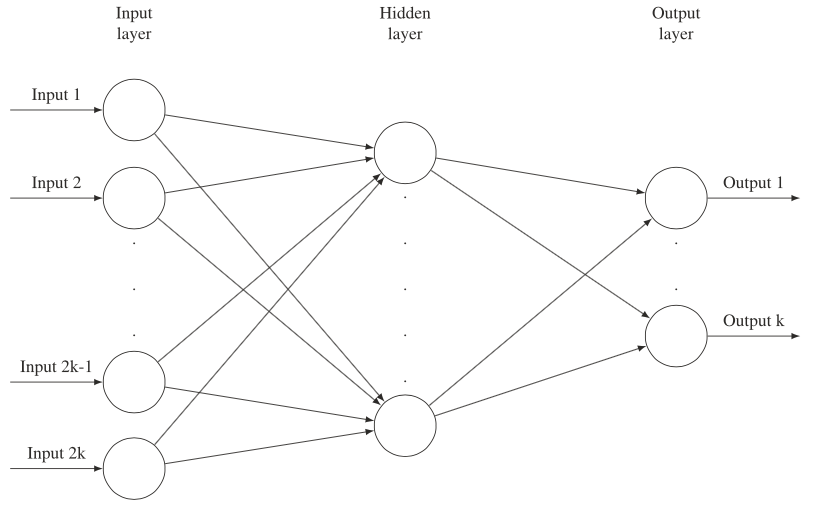
\epsfig{file=images/neural_network_topology.png, width=10cm}
					\caption{Topology of the ANN}
					\label{fig:neural_network_topology}
				\end{figure}	
				Since the main goal is to enhance the fairness experienced at the network as a whole, the minimization function used considers both performance and fairness. The authors also described the processes of data collection, training, testing and optimization, as well as the update phase. Basically, information for training/testing is constantly being updated to run the optimization, which error results are back-propagated to the previous levels. In case that the MSE (Mean Squared Error) and the desired fail number ratio ($\text{FNr}_{des}$) are below the expected results, the changes are applied and the process ends. Otherwise, both MSE and learning rate $\mu$ are decreased before running a new iteration (or epoch) of the whole process. Simulations show the performance of the ANN approach in three different scenarios: exposed-node,  hidden-node, and high-density (7 APs and 8 STAs per AP). In all the cases, both aggregate throughput and fairness are shown to be enhanced after few epochs. In the high-density case, the gain noticed in the aggregate throughput exceeds the 45\%, while fairness starts from 0.5 and ends up to 0.7.

				Table \ref{tbl:rl_wns} shows a summary of the State-of-the-art in RL applied to spatial reuse in WNs.
				\begin{table}[h!]
				\centering
				\resizebox{\textwidth}{!}{\begin{tabular}{|c|l|c|l|l|}				
						\hline
						\multicolumn{1}{|c|}{\textbf{Work}} & \multicolumn{1}{c|}{\textbf{Presented Approach}} & \textbf{\begin{tabular}[c]{@{}c@{}}Centralised/\\ Decentralised\end{tabular}} & \multicolumn{1}{c|}{\textbf{Positive Aspects}} & \multicolumn{1}{c|}{\textbf{Negative Aspects}} \\ \hline
						\cite{nie1999q} & \begin{tabular}[c]{@{}l@{}}Q-learning for channel\\assignment in mobile\\ communications\end{tabular} & \begin{tabular}[c]{@{}l@{}}Decentralized\end{tabular}  &  \begin{tabular}[c]{@{}l@{}}$\bullet$  Partially decentralised\\$\bullet$ Shows learning feasibility\\in WNs\end{tabular} & \begin{tabular}[c]{@{}l@{}}$\bullet$ Communication overhead\\is not considered\\ $\bullet$ Q-learning parameters \\are deterministically set\end{tabular}  \\ \hline	
						\cite{li2009multi} & \begin{tabular}[c]{@{}l@{}}Q-learning for channel\\assignment in multi-agent\\environments\end{tabular} & \begin{tabular}[c]{@{}l@{}}Decentralized\end{tabular}  &  \begin{tabular}[c]{@{}l@{}}$\bullet$  Fully decentralised\\$\bullet$ Considers multi-agent\\scenarios\end{tabular} & \begin{tabular}[c]{@{}l@{}}$\bullet$ Very limited scenario\\$\bullet$ Equilibrium is easy\\ to reach\end{tabular}  \\ \hline	
						\cite{bennis2010q} & \begin{tabular}[c]{@{}l@{}}Q-learning for channel\\assignment in femtocell\\networks\end{tabular} & \begin{tabular}[c]{@{}l@{}}Decentralized\end{tabular}  &  \begin{tabular}[c]{@{}l@{}}$\bullet$  Fully decentralised\\$\bullet$ The rewarding system\\is more accurate for\\wireless communications\end{tabular} & \begin{tabular}[c]{@{}l@{}}$\bullet$ Very limited scenario\\$\bullet$ Q-learning parameters \\are deterministically set\end{tabular}  \\ \hline		
						\cite{maghsudi2015joint} & \begin{tabular}[c]{@{}l@{}}MABs for D2D \\channel allocation\\ and transmit power\\adjustment\end{tabular} & Decentralised & \begin{tabular}[c]{@{}l@{}} $\bullet$ Proves regret minimisation \end{tabular}  &  \begin{tabular}[c]{@{}l@{}} $\bullet$ Simple scenario\\ $\bullet$ Cases in which correlated\\equilibria cannot be reached\\are not studied \end{tabular}\\ \hline	
						\cite{maghsudi2015channel} & \begin{tabular}[c]{@{}l@{}}MABs for D2D \\channel allocation\end{tabular} & Decentralised & \begin{tabular}[c]{@{}l@{}}$\bullet$ Interesting approach \\for inferring the others'\\behaviour \end{tabular}  &  \begin{tabular}[c]{@{}l@{}} $\bullet$ Simple scenario \\$\bullet$ Convergence can be easily\\ reached \end{tabular}\\ \hline					
						\cite{jamil2016novel} & \begin{tabular}[c]{@{}l@{}}ANN for adjusting the \\transmit power and the \\carrier sense threshold \\of all the devices in a \\wireless network\end{tabular} &  Centralised & \begin{tabular}[c]{@{}l@{}}$\bullet$ Powerful method \\to improve network\\ performance\end{tabular}  &  \begin{tabular}[c]{@{}l@{}} $\bullet$ Full control is required\\ $\bullet$ Only applicable to fully \\centralised scenarios\end{tabular}\\ \hline	
				\end{tabular}}
				\caption{State-of-the-Art of Reinforcement Learning for spatial reuse in Wireless Networks}
				\label{tbl:rl_wns}
			\end{table}	
	
	%%%%%%%%%%%%%%%%%%%%%%%%%%%%%%%%%%%%%%%
	% ONGOING WORK			        					   %%%%%%%%%%%%%
	%%%%%%%%%%%%%%%%%%%%%%%%%%%%%%%%%%%%%%%	
	\chapter{Current Contributions and Ongoing Work}
	\label{section:current_contributions}
		In this Section we describe the current contributions done during the first year, as well as the ongoing research activity and the preliminary results.

		\section{Wireless Networking Through Learning}
		\label{section:mdm}		
			Through the \textit{Wireless Networking Through Learning} project, which is under the \textit{Mar\'ia de Maeztu excellence program}, the following contributions have been done:
			\begin{itemize}
				\item A conference paper was submitted to the IEEE International Symposium on Personal, Indoor and Mobile Radio Communications (PIMRC) \cite{wilhelmi2017implications}.
				\item A journal article was prepared for future submission to the Computer Networks journal \cite{wilhelmi2017enhancing}.\footnote{\url{https://www.journals.elsevier.com/computer-networks/}}
				\item An extension of \cite{wilhelmi2017enhancing} and \cite{wilhelmi2017implications} is being developed for exploring centralized approaches and to provide a more realistic simulation.
				\item A journal article in collaboration with the Artificial Intelligence and Machine-Learning Research Group (AI-ML) is under construction \cite{bellalta2017learning}.
				\item A poster was presented on the 5th PhD Doctoral Workshop, held at the UPF \cite{wilhelmi2017improving}.
				\item We are actively collaborating in a journal article \cite{barrachina2017ctmn}.
				\item A collaboration agreement was achieved with the Wireless Communications department at Universidad Aut\'onoma Nacional de M\'exico (UNAM). The subject of this collaboration is to work in a publication that considers the inference of the coexistent devices configurations for allowing intelligent self-adjustment in dense WNs.
			\end{itemize}	
			
		\section{Other Projects}
		\label{section:other_projects}	
			To support the main research activity, some other projects are being under development, which are detailed in this section.
			
			\subsection{Analytical Models and Simulators}
			\label{section:validation}	
				A fundamental task for this Thesis is to properly understand and/or develop the most suitable simulation tools, which will allow us validating the results obtained from the research activity. One of the most important analytical models to compute the throughput in an overlapping network is the Continuous Time Markov Networks (CTMNs) model \cite{bellalta2014throughput}, which captures the operation of the CSMA/CA protocol. In relation to CTMNs, we have started a collaboration for developing a framework that is able to build the Markov chains for analytical throughput calculation, according to the nodes input (many features such as the position, the power transmitted or the channel bonding policy are taken into consideration). The project is leaded by Sergio Barrachina \cite{barrachina2017ctmn}. Another important analytical model for throughput calculation in overlapping WLANs is the Bianchi's model \cite{bianchi2000performance}. The Bianchi's model is a benchmark in the current literature that we aim to use for validating the Komondor simulator (further described in Section \ref{section:cisco_project}).				
				
				Regarding network simulators, we highlight ns-3 \cite{carneiro2010ns}, which is widely spread in the wireless community. However, the learning curve is high and many novel features are not yet supported. 	Other available simulators are ns-2 \cite{issariyakul2011introduction}, OPNET \cite{modeler2009opnet} or Omnet++ \cite{varga2008overview}.
				
			\subsection{Development of an IEEE 802.11ax Event-Based Simulator}
			\label{section:cisco_project}				
				In order to perform simulations based on the IEEE 802.11ax standard, we have started building our own event-based simulator for WLANs, which has been called Komondor \cite{barrachina2017komondor}. Besides being a useful tool for supporting most of the research activity performed along the Thesis, the Komondor simulator is also the result of a collaboration with Cisco. Komondor is built on top of COST \cite{chen2005sense}, which provides the baseline for synchronised messages exchanging. The decision of building a simulator, apart from the Cisco's collaboration, lies in the impediments shown by other simulators such as Network Simulator 3 (ns-3), which does not include many of the novel features provided by the IEEE 802.11ax standard, and which are the main matter of this Thesis. Moreover, building these functionalities in ns-3 is an extremely costly task, not only because of the complexity of the program, but for the significant learning curve. At the present time, Komondor v1.0 has been released and successfully validated against the well-known Bianchi's model for overlapping WLANs. Its main features are the Request to Send / Clear to Send (RTS/CTS) IEEE 802.11 mechanism, CSMA/CA with exponential slotted binary backoff (BEB), configurable packet traffic generation, collision type identification through logical events, and detailed statistics for metrics of interest such as average throughput per WLAN or detected hidden nodes. The code\footnote{\url{https://github.com/wn-upf/Komondor}} is open for dissemination and improvement requests.
				
			\subsection{AP Association and Self-Managed Networks through Learning}
			\label{section:fon_project}	
				We are also expected to contribute in the collaboration Fon-UPF, which is based in two main projects for improving network performance in coexistent wireless scenarios. Fon is a company that has built the world's largest network made up of people sharing their Wi-Fi. Due to new requirements in wireless networks and the increasing density in their main deployment scenario (residential buildings), Fon aims to enhance the AP association and autonomous management processes through Machine Learning techniques. For the former, a mobile application provided to users is used to gather information about the surrounding Fon networks, which is sent to a central unit. The latter must decide which is the best network for making user association. Secondly, to further improve networks performance, an autonomous system for management is aimed to be developed. In this case, the gathered information for decision-making is also retrieved from the APs. The core idea is to empower the system with the necessary intelligence to allow self-adjustment in the Wi-Fi networks, so that the interference can be minimised along the network, thus maximising fairness and throughput.
			
		\section{Preliminary Results}
		\label{section:preliminary_results}	
			The research activity performed during the first year was mainly focused on understanding network interactions (emphasising dense deployments), as well as to open discussion about the usage of RL in WNs. In \cite{wilhelmi2017implications}, we applied Q-learning in a decentralised manner to the resource allocation problem in dense WNs. We showed that the best-performing actions that enhance the aggregate throughput can be found through RL. In the presented adversarial scenario (4 WNs compete for accessing to 2 overlapping channels), the most probable actions after applying Q-learning turn to be the ones that use a higher transmit power (Figure \ref{fig:ql_actions}). Despite resulting into a fair resources distribution (Figure \ref{fig:ql_avg_tpt}), such aggressive adversarial setting leads to a high variability in the throughput experienced by the individual networks (Figure \ref{fig:ql_performance}). Hence, the favourite actions provide intermittent good/poor performance depending on the neighbouring decisions. 		
			\begin{figure}[h!]
				\centering
				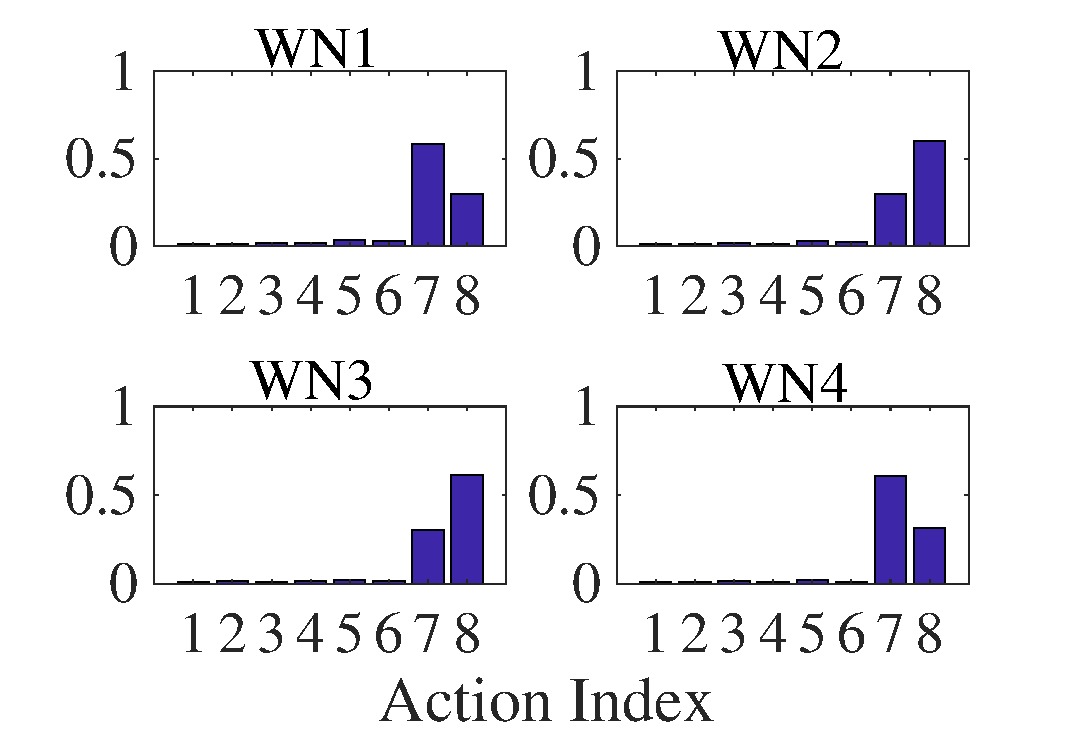
\epsfig{file=images/e_1_a1_g095.eps, width=8cm}
				\caption{Probability of choosing an action in each overlapping WN \cite{wilhelmi2017implications}}
				\label{fig:ql_actions}
			\end{figure}
			\begin{figure}[t!]
				\centering
				\begin{subfigure}[b]{0.4\textwidth}
					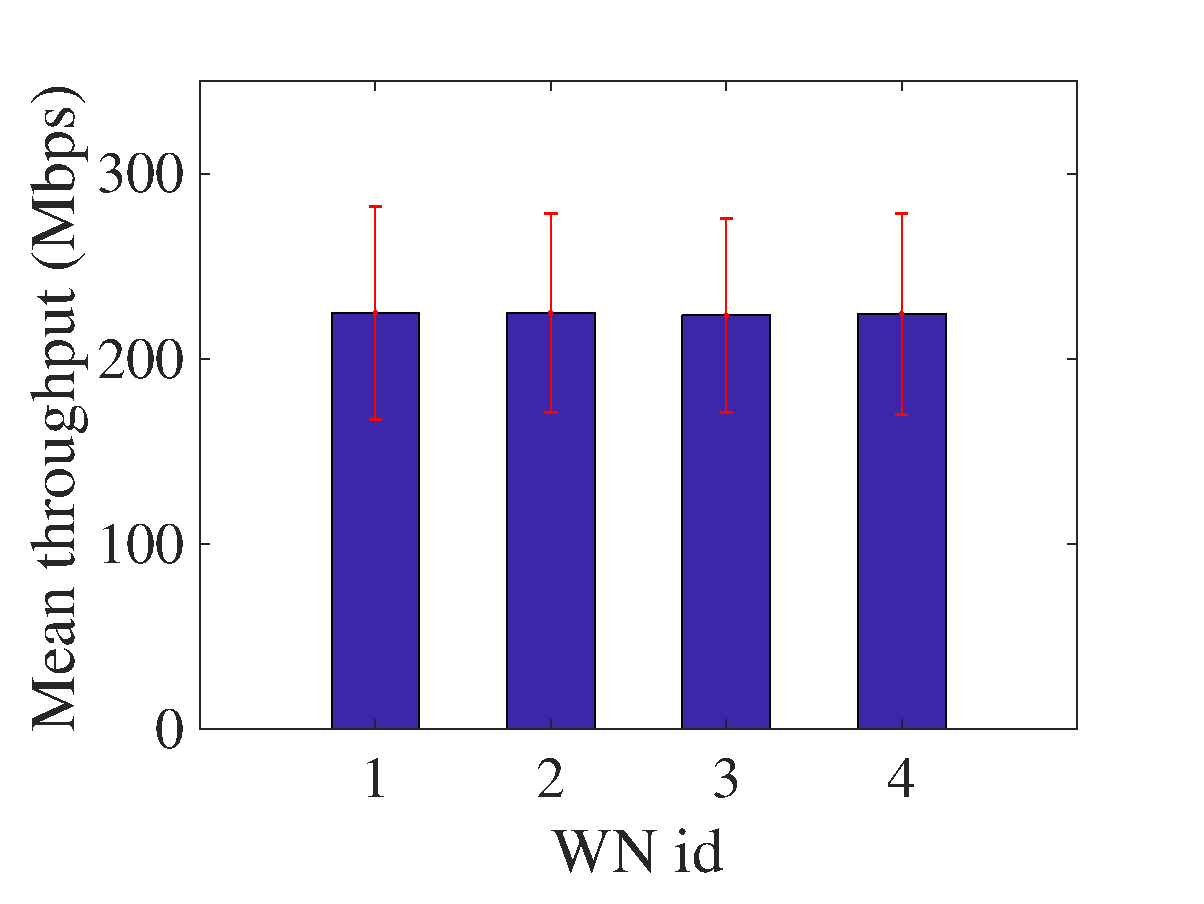
\includegraphics[width=\textwidth]{images/e_1_a1_g095_avg_tpt}
					\caption{Average throughput}
					\label{fig:ql_avg_tpt}
				\end{subfigure}
				\begin{subfigure}[b]{0.4\textwidth}
					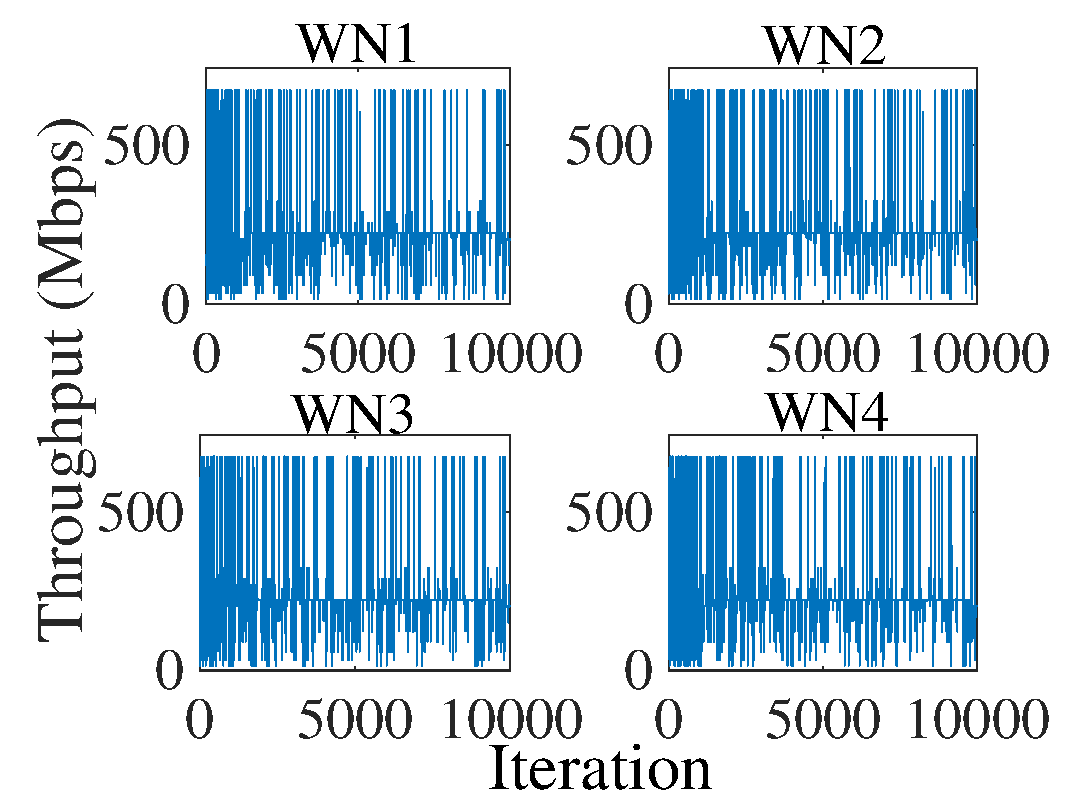
\includegraphics[width=\textwidth]{images/e_1_a1_g095_ind_tpt}
					\caption{Temporal throughput}
					\label{fig:ql_temporal_tpt}
				\end{subfigure}		
				\caption{Individual performance experienced by each overlapping WN on applying decentralised Q-learning \cite{wilhelmi2017implications}}
				\label{fig:ql_performance}
			\end{figure}
		
			An extension of \cite{wilhelmi2017implications} is provided in \cite{wilhelmi2017enhancing}, in which several Multi-Armed Bandits techniques are compared to solve the same situation. Each algorithm is extensively analysed to study the actual role of each parameter (exploration, learning rate...) into network performance and interactions. Furthermore, it is shown that maximizing the individual throughput based on local information only, leads to a solution very close to the optimal proportional fairness.			
			
			Finally, to cover the centralised case, we have repeated the same experiments but using a shared reward, so that convergence can be speeded up. For that, some preliminary simulations are carried out to consider the proportional fairness\footnote{The proportional fairness is the logarithmic sum of the individual throughputs of each node.} as the reward used by all the overlapping nodes. As shown in Figure \ref{fig:ql_performance_centralised}, the variation of the temporal throughput is much lower (\ref{fig:proportional_fairness_qlearning_ind_tpt}), at the expense of providing a lower fairness (\ref{fig:proportional_fairness_qlearning_avg_tpt}). However, the fact of suffering a certain unfairness may result acceptable, specially in asymmetric scenarios where few nodes are in a less favourable position.
			\begin{figure}[t!]
				\centering
				\begin{subfigure}[b]{0.4\textwidth}
					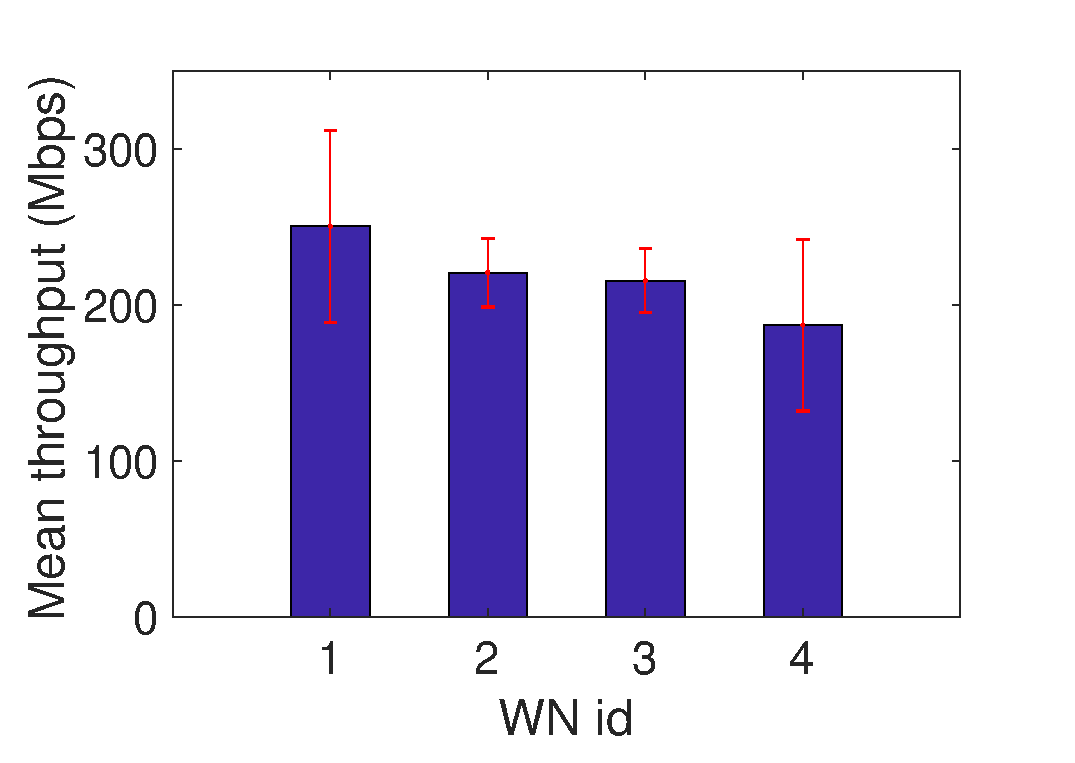
\includegraphics[width=\textwidth]{images/proportional_fairness_qlearning_avg_tpt}
					\caption{Average throughput}
					\label{fig:proportional_fairness_qlearning_avg_tpt}
				\end{subfigure}
				\begin{subfigure}[b]{0.4\textwidth}
					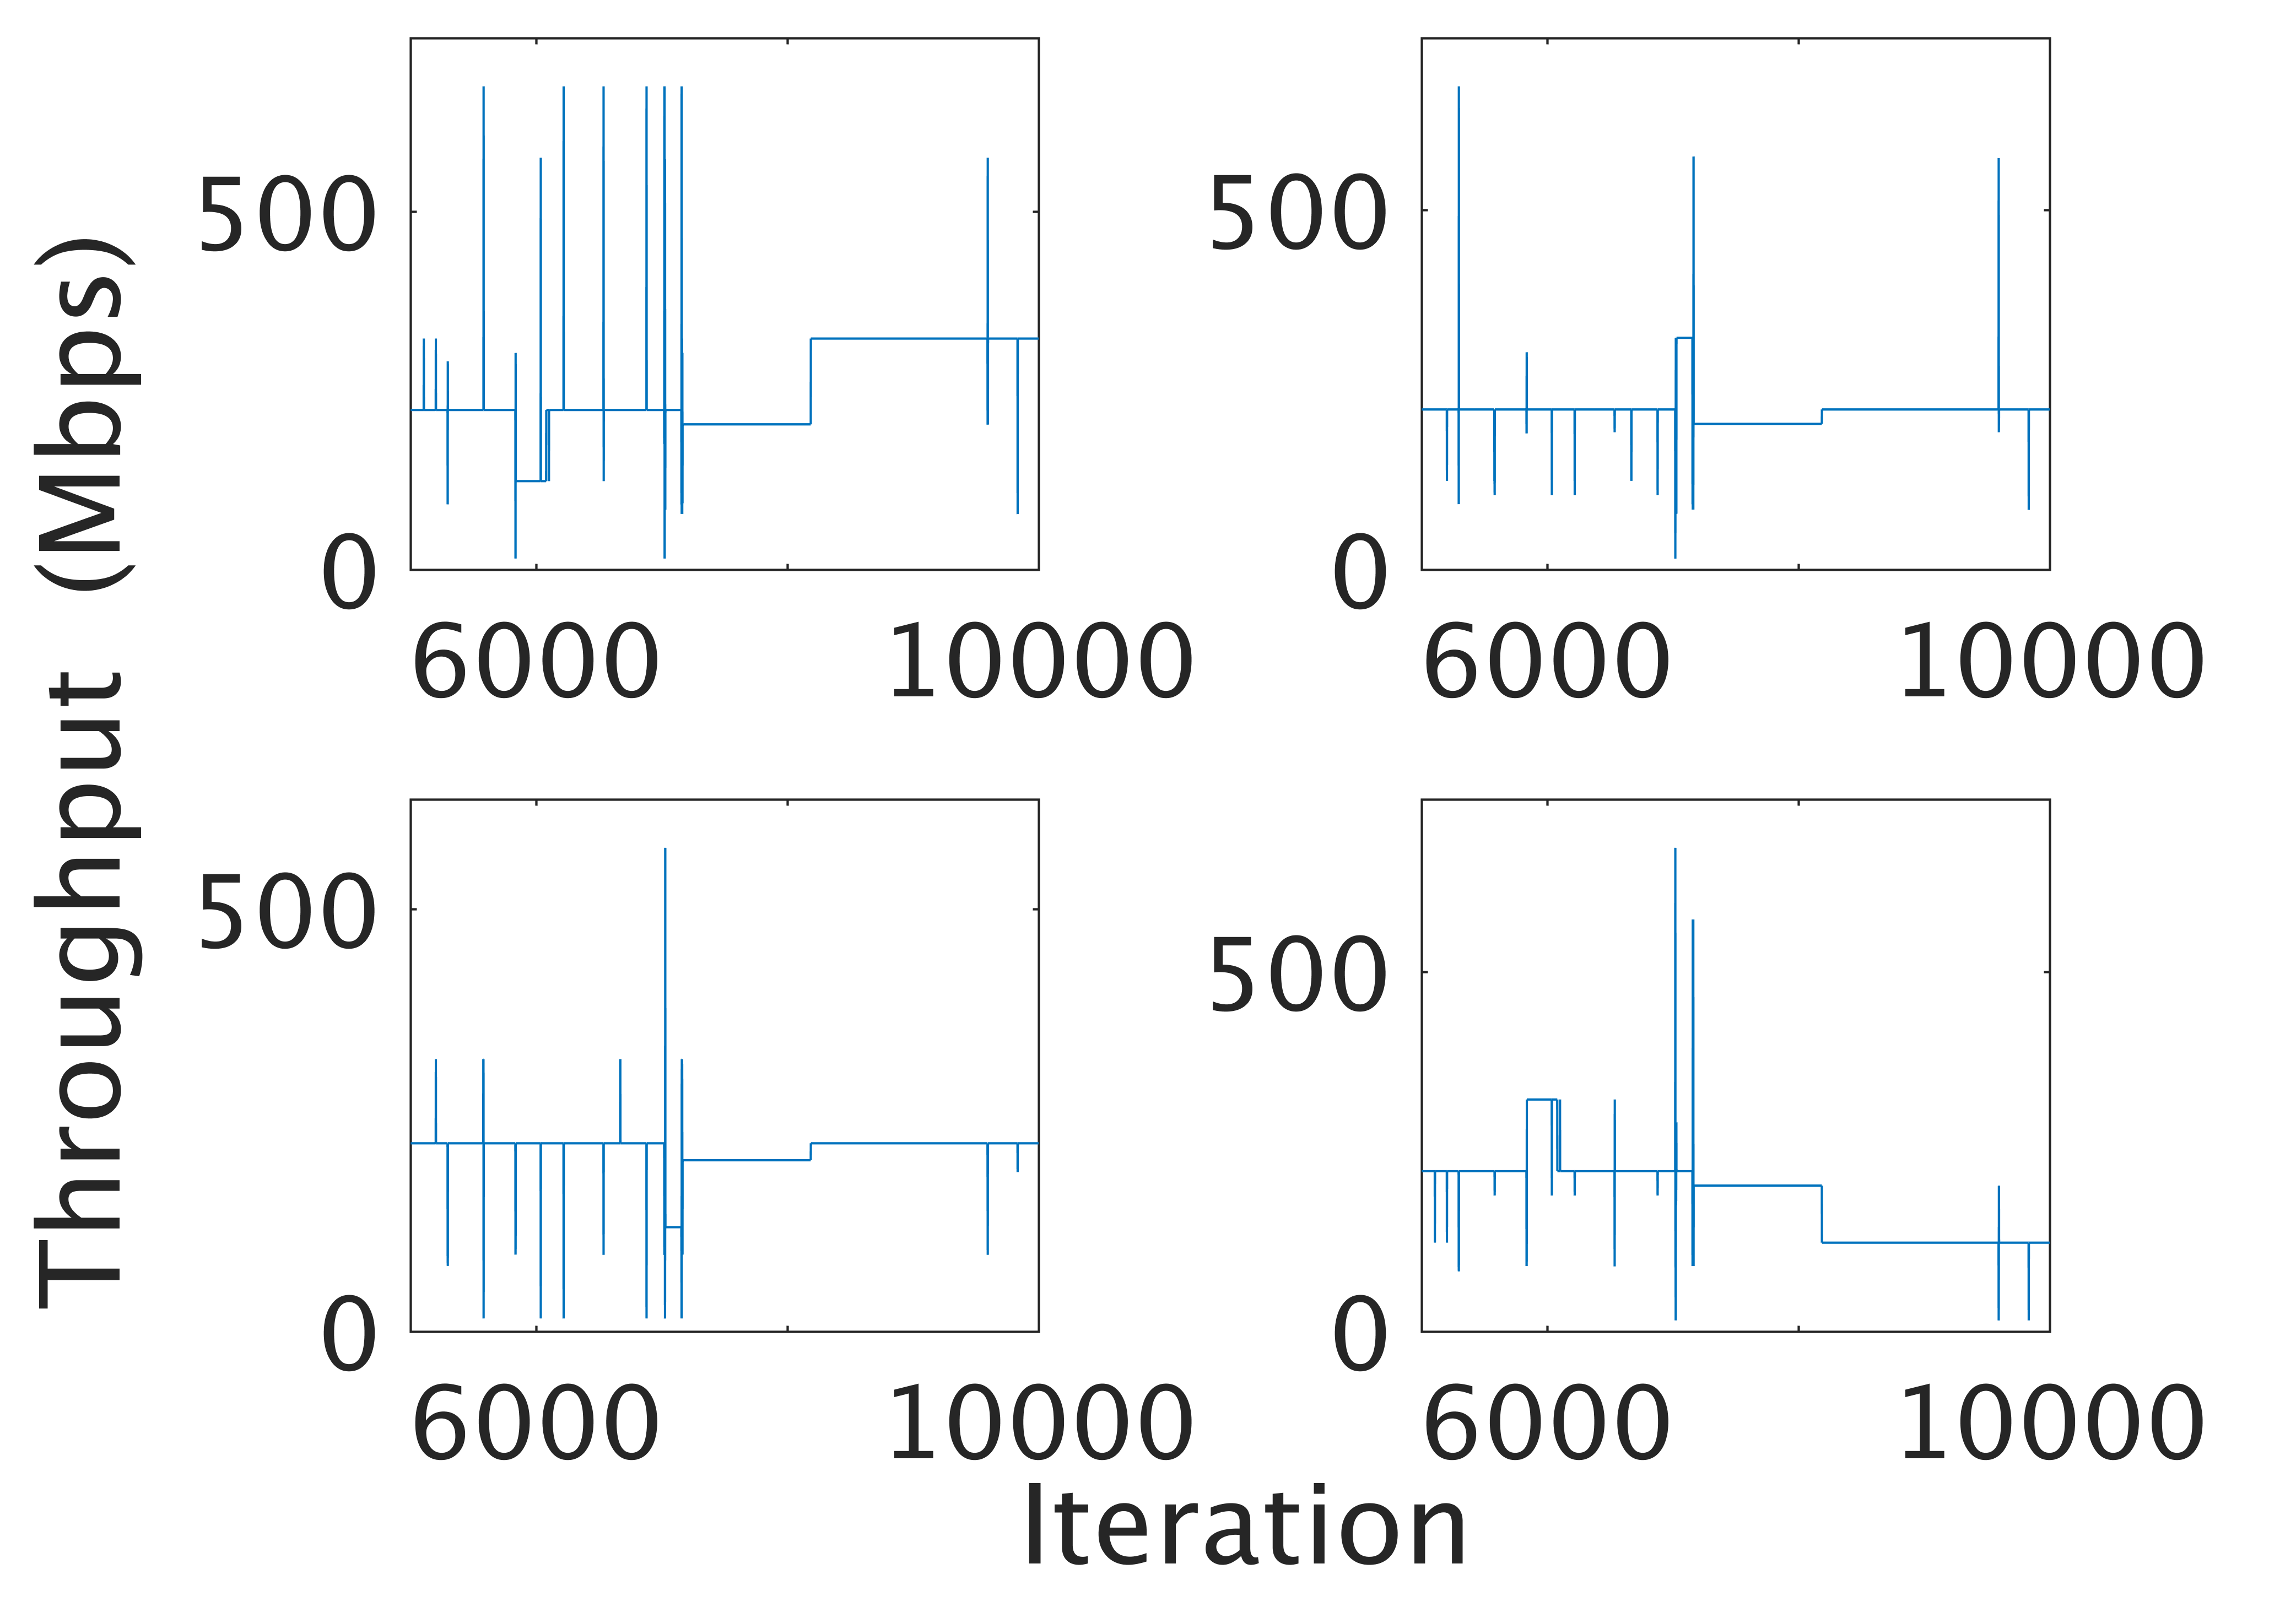
\includegraphics[width=\textwidth]{images/proportional_fairness_qlearning_ind_tpt}
					\caption{Temporal throughput}
					\label{fig:proportional_fairness_qlearning_ind_tpt}
				\end{subfigure}		
				\caption{Individual performance experienced by each overlapping WN on applying centralised Q-learning}
				\label{fig:ql_performance_centralised}
			\end{figure}
			

	%%%%%%%%%%%%%%%%%%%%%%%%%%%%%%%%%%%%%%%
	% FUTURE WORK										   %%%%%%%%%%%%%
	%%%%%%%%%%%%%%%%%%%%%%%%%%%%%%%%%%%%%%%	
	\chapter{Planning and Future Work}
	\label{section:future_work}
		
		%\section{Objectives and Tasks}
		%\label{section:objectives}
		We have put forward a range of objectives to be accomplished during the development of the research activities related to this Thesis, which are listed below together with the involved tasks:
		\begin{itemize}
			\item \textbf{Objective 1 (O1):} Understanding the dynamics of coexistent WNs when competing for bandwidth resources, as well as obtaining an extensive knowledge on the current techniques used for improving the spatial reuse in wireless networks.
			\begin{itemize}
				\item Extension of the current work in decentralised learning implications (DL1): Application of CTMN Framework to the work presented in \cite{wilhelmi2017implications}. Extend it to provide the centralised perspective.
				\item Make a publication collecting these techniques to provide an State-of-the-Art to the resource allocation problem in wireless networks (SOA1).
				\item Internship in Mexico (UNAM): Reinforcement Learning with Neighbouring Performance Inference for Resource Allocation in High-Density WLANs (UN1), which aims to study channel estimation and inference techniques to envision the behaviour of an overlapping WN from a decentralised point of view.
				\item Extrapolate the work done regarding RL in WNs in order to capture dynamics in terms of user and traffic variability (RL2). Understanding network dynamics and future requirements for dense wireless networks.
			\end{itemize}
			\item \textbf{Objective 2 (O2):} Understanding analytical and simulation tools for WNs performance computation.
			\begin{itemize}
				\item Komondor simulator: launch versions 2.1 (KM1) and 2.2 (KM2) that include intelligent agents to boost the network performance. Also, write a technical report to be published (KM3).
				\item CTMN framework collaboration with Barrachina: provide a framework to compute network throughput through the CTMN model (CTMN1).
			\end{itemize}	
			\item \textbf{Objective 3 (O3):} Understanding the RL techniques that better suit the resource allocation problem in WNs. Study also the basics on Game Theoretical and Adversarial settings.
			\begin{itemize}
				\item Make a publication reviewing several techniques to prove their efficiency when applied in the wireless communications field (RL1).
				\item Make a publication summarizing all the work done during the Thesis, which provides a ML-based solution to the resource allocation problem in future WLANs (RL2). Providing ML-based solutions to the resource allocation problem in future WLANs.
			\end{itemize}	
			\item \textbf{Objective 4 (O4):} In parallel, through the FON collaboration, we find a set of tasks that differ from the main research line of this Thesis, but which provide complementary knowledge and enrich the degree of expertise in other fields.
			\begin{itemize}
				\item Acquire the necessary knowledge to face the AP association problem in WNs from both decentralised and centralised perspectives. Thus, provide a State-of-the-Art in the field (FON1).
				\item Acquire the necessary knowledge for self-adjustment in WNs Thus, provide a State-of-the-Art in the field (FON2).
			\end{itemize}		
		\end{itemize}
	
%		\section{Gantt Diagram}
%		\label{section:gantt}
%		To provide a better visualization of the development of the tasks presented in Section \ref{section:objectives}, we provide the following Gantt diagram:
%			
%		\noindent\resizebox{\textwidth}{!}{
%			\begin{tikzpicture}[x=.5cm, y=1cm]
%				\begin{ganttchart}[vgrid,hgrid]{1}{24}
%					\gantttitle{2017}{3} \gantttitle{2018}{12} \gantttitle{2019}{9}\\
%					\gantttitlelist{10,...,12}{1} \gantttitlelist{1,...,12}{1} \gantttitlelist{1,...,9}{1} \\
%					% 
%					\ganttgroup{DL1}{1}{5} \\
%					\ganttgroup{SOA1}{1}{5} \\
%					\ganttgroup{UN1}{1}{5} \\
%					\ganttgroup{RL1}{1}{5} \\
%					\ganttmilestone{O1}{5} \ganttnewline
%					% 
%					\ganttgroup{KM1}{1}{2} \\
%					\ganttgroup{KM2}{1}{2} \\
%					\ganttgroup{KM3}{1}{2} \\
%					\ganttgroup{CTMN1}{1}{2} \\
%					\ganttmilestone{O2}{2} \\		
%					% 
%					\ganttgroup{ML1}{1}{2} \\
%					\ganttgroup{ML2}{1}{2} \\
%					\ganttmilestone{O3}{2} \\		
%					% 
%					\ganttgroup{FON1}{3}{8} \\
%					\ganttgroup{FON2}{3}{8} \\
%					\ganttmilestone{O4}{8} \ganttnewline
%					% 
%				\end{ganttchart}
%			\end{tikzpicture}
%		}	
	
	%%%%%%%%%%%%%%%%%%%%%%%%%%%%%%%%%%%%%%%
	% BIBLIOGRAPHY					      				   %%%%%%%%%%%%%
	%%%%%%%%%%%%%%%%%%%%%%%%%%%%%%%%%%%%%%%	
	\bibliographystyle{unsrt}
	\bibliography{bib}

\end{document}